\documentclass[11pt,a4paper]{article}

\usepackage[margin=1.1in]{geometry}
\usepackage{amsmath,amssymb,amsthm,mathtools}
\usepackage[T1]{fontenc}
\usepackage{microtype}
\microtypesetup{expansion=false}
\usepackage{tikz}
\usetikzlibrary{positioning,arrows.meta,calc,fit,backgrounds,patterns}
\usepackage{booktabs}
\usepackage{listings}
\usepackage{stmaryrd}
\usepackage[hidelinks]{hyperref}
\usepackage{enumitem}

\theoremstyle{plain}
\newtheorem{theorem}{Theorem}
\newtheorem{proposition}[theorem]{Proposition}
\newtheorem{lemma}[theorem]{Lemma}
\newtheorem{corollary}[theorem]{Corollary}
\newtheorem{conjecture}[theorem]{Conjecture}
\theoremstyle{definition}
\newtheorem{definition}[theorem]{Definition}
\newtheorem{observation}[theorem]{Observation}
\newtheorem{example}[theorem]{Example}
\theoremstyle{remark}
\newtheorem{remark}[theorem]{Remark}

\newcommand{\rhoc}{\textsf{rho}}
\newcommand{\Nil}{\mathbf{0}}
\newcommand{\sepc}{\mathbin{\big|}}
\newcommand{\Hq}{\mathsf{H}}
\newcommand{\out}{\mathsf{out}}
\newcommand{\inn}{\mathsf{in}}
\newcommand{\Rnn}{\mathbb{R}_{\geq 0}}
\newcommand{\Cx}{\mathbb{C}}
\newcommand{\Terms}{\mathcal{T}}
\newcommand{\Cfg}{\mathcal{C}}
\newcommand{\Wt}{\mathcal{W}}
\newcommand{\Red}{\mathrm{Red}}
\newcommand{\prop}{\mathbf{a}}
\newcommand{\wmap}{w}
\newcommand{\dpt}{d}
\newcommand{\gfac}{g}
\newcommand{\funds}{\mathrel{\vdash_{\!\$}}}
\newcommand{\class}{\mathrm{cls}}
\newcommand{\Lop}{L}
\newcommand{\Heff}{H_{\mathrm{eff}}}
\newcommand{\dbr}[1]{\llbracket #1 \rrbracket}

\lstdefinestyle{rho}{
  basicstyle=\ttfamily\footnotesize,
  keywordstyle=\bfseries,
  commentstyle=\itshape,
  morekeywords={new,in,for,contract,match,if,else,true,false,Nil,where,and,or,not,
                exists,forall,nu,rules,rewrites,equations,types,language,name},
  morecomment=[l]{//},
  columns=fullflexible,
  breaklines=true,
  breakatwhitespace=false,
  showstringspaces=false,
  frame=none,
  xleftmargin=1em
}
\lstset{style=rho}

\title{\textbf{Weighted Graph-Structured Lambda Theories}\\[0.4em]
\large Stochastic and quantum execution for MeTTaIL, with a spiking\\
recurrent network as a worked example}
\author{A F1R3FLY.io working note}
\date{August 2026 \\[0.2em]\small Second version, revised in response to referee comments}

\begin{document}
\maketitle

\begin{abstract}
We equip the rewrite rules of a finitely presentable graph-structured lambda theory (GSLT), as
presented in MeTTaIL, with \emph{weight maps}: finite maps whose keys are spatial--behavioural
formulae refining the left-hand side of a rule and whose values are weights. A weight map instance
is part of a state specification, so a rewrite may update it; weights are therefore dynamic. We
develop the construction in three movements. First, we impose a \emph{partition discipline} on the
key set --- the refinements of a rule's left-hand side must be pairwise exclusive and jointly
exhaustive --- and show that this single requirement is what makes the weighting a total,
single-valued classification of redexes; we then say what it costs, which is a dilemma rather than a
theorem: a partition stated inside the generated logic demands Boolean structure of the target
specification, and a partition stated outside it forfeits specification closure. Second, with
weights in $\Rnn$ we define propensity as $\prop = \wmap(\varphi)\cdot\sum_k \gfac(k)$ over
classified, funded redex positions and obtain a Gillespie simulator; we prove that the construction
restricted to the summation-free $\pi$-calculus, static maps, and channel-identity keys is exactly
the Stochastic Pi Machine, and that dynamic maps take it strictly beyond. Third, with weights in
$\Cx$ --- read not as a second semiring instance but as amplitudes, with $\lambda(z) = |z|^2$ the
rate an amplitude denotes --- we read each refinement entry as a Lindblad jump operator over a basis
of reachable \emph{configurations}, terms paired with weight maps, which is what keeps the generator
fixed under plasticity. This gives a quantum continuous-time Markov chain in the sense of Xu, Mei,
Guan and Yu, of which the Gillespie algorithm is the quantum-jump unravelling at zero Hamiltonian.
Fixing the normalisation of a jump channel by conservativity over the classical chain --- a channel's
amplitude is the square root of its aggregate rate --- recovers the classical chain exactly as the
$|z|^2$ marginal, disposes of an apparent superlinearity in reactant multiplicity, and locates all
coherence in the Hamiltonian, which the un-quotiented part of the equational theory supplies. The
worked example is an asynchronous stochastic spiking recurrent network in a weighted \rhoc\ theory:
neurons are persistent for-comprehensions, synaptic efficacies live in the weight map rather than in
the payload, thresholds are join structure, a saturating response emerges from the chain rather than
being written into a term, and a minimal local Hebbian potentiation rule is exactly the refinement
entries' update functions --- so that learning and inference are the same transition relation,
differing only in which component of the state they touch.
\end{abstract}

\tableofcontents

\section{Introduction}
\label{sec:intro}

A rewrite rule's left-hand side is a type. Terms inhabit it; the rule fires at its inhabitants. This
note is about what happens when one refines that type and attaches a number to each refinement.

The move is small to state and consequential to develop. A GSLT is a triple $(\Sigma, E, R)$: a
signature which is in general a lambda theory, a set of equations imposing a structural congruence,
and an adjoined graph of rewrite rules \cite{omnibus}. Given such a presentation, the OSLF family of
algorithms generates a logic from it, with one structural connective per term former of $\Sigma$ and
one context-labelled modality per rule of $R$ together with a choice of redex position
\cite{omnibus,classifier}. The formulae of that generated logic are exactly the vocabulary in which
one can refine a rule's left-hand side --- and they are generated, not designed, so the refinements
come for free with the theory. To weight a rule is to give a finite map
\[
\varphi_1 \mapsto v_1, \quad \ldots, \quad \varphi_m \mapsto v_m
\]
from such refinements to weights. A term's redexes are then classified by which refinement they
satisfy, and the weights turn the set of enabled redexes into a distribution.

Two things distinguish this from the existing literature on stochastic process calculi.

\paragraph{Keys are formulae, not names.} In Priami's stochastic $\pi$-calculus \cite{priami} and in
Phillips and Cardelli's Stochastic Pi Machine (SPiM) \cite{spim,spim-sim}, a rate is attached to a
\emph{channel}. That is one refinement among many: ``this redex is a communication on $n$'' is a
particular formula in the generated logic, and there is no reason the modeller should be restricted
to it. Once keys are formulae, a rate may depend on the shape of the payload, on the \emph{namespace}
a channel belongs to --- which in a reflective calculus is real structure, reachable by the classifier
through the name predicate $@\varphi$, and is what lets one key cover a growing population of
channels (\S\ref{sec:rnn-uniform}) --- or on any Boolean combination of these. Channel identity is
recovered as the degenerate case (\S\ref{sec:spim}). We are careful not to claim more than that. The
classifier of Proposition~\ref{prop:classify} evaluates its formula at the matched left-hand side
$L\sigma$ and not at $k[L\sigma]$, so the ambient context is not visible to a key at all; properties
of a redex's \emph{position} are the business of the geometric factor $\gfac(k)$ (\S\ref{sec:geometric}),
and the division of labour between the two is clean only because it is respected.

\paragraph{Maps are state, not declaration.} A weight map instance is part of a state
specification. A rule's refinement entries therefore carry not only a weight but an \emph{update
function} on the whole map, applied when the rule fires. Rates change during execution. SPiM does
not permit this --- its rates are fixed at declaration --- and the restriction is not incidental to
its design but constitutive of it, since a static rate function is what makes the underlying object
a time-homogeneous CTMC over terms alone. We recover Markovianity by a different route: the weight
map is \emph{in} the state, so the chain is over configurations $(P, \wmap)$ rather than over terms
(\S\ref{sec:gillespie}). This is the technical content of ``the map may be updated,'' and it is what
the worked example of \S\ref{sec:rnn} needs, because plasticity is nothing other than a weight-map
update.

Two further points of scope. The construction is generic over the GSLT: it applies to any theory
one can write down in MeTTaIL's \texttt{language!} block \cite{mettail}, so one obtains a stochastic
machine for the ambient calculus, for a user-defined DSL, or for the \rhoc\ calculus, by writing the
theory rather than by writing a simulator. And the weight codomain is a parameter. We treat two
instances: $\Rnn$, giving classical Gillespie simulation (\S\ref{sec:gillespie}); and $\Cx$, giving
a quantum continuous-time Markov chain in the sense of \cite{qctmc} and a Gillespie-inspired
trajectory simulation for it (\S\ref{sec:quantum}). A third instance --- weights in a quantale,
giving a fuzzy calculus --- is deliberately out of scope here; see \cite{fuzzy}.

\paragraph{What is new.} Beyond the two distinguishing points above:
\begin{enumerate}[label=(\roman*),leftmargin=2.2em]
\item The \emph{partition discipline} of \S\ref{sec:refinement}, and the observation that it is not
a technicality but the condition under which weighting is well defined at all --- together with an
account of what it costs, namely that stating it internally demands Boolean structure of the target
logic specification while stating it externally forfeits specification closure
(\S\ref{sec:boolean}).
\item A propensity formula (\S\ref{sec:propensity}) that separates four factors which the literature
usually conflates: the refinement's weight, a geometric factor accumulated up the context rules,
redex multiplicity, and a funding gate supplied by cost accounting.
\item Theorem~\ref{thm:spim}: the summation-free fragment of SPiM is the construction's restriction,
exactly.
\item The normalisation result of \S\ref{sec:bosonic}, which fixes what a quantum jump channel is by
requiring the complex construction to be conservative over the real one, and thereby settles a
question that the first version of this note left open.
\item Theorem~\ref{thm:jump-gillespie}: the Gillespie algorithm is the quantum-jump unravelling at
zero Hamiltonian --- so ``Gillespie-inspired'' is a theorem about degeneration, not an analogy. Under
\S\ref{sec:bosonic} it needs no hypothesis on the jump structure.
\item The observation (\S\ref{sec:qctmc-logic}) that the OSLF-generated formulae supply exactly the
atomic propositions that quantum CTMC model checking otherwise has to be handed by hand.
\item The spiking-network example of \S\ref{sec:rnn}, whose thesis is that \emph{synaptic efficacy is
represented as transition intensity in the operational semantics, and the same transition updates
that intensity}: the efficacies live in the weight map, the threshold lives in the join structure of
a for-comprehension, a saturating response is emergent, and learning is a weight-map update
performed by the same rewrite that performs inference.
\end{enumerate}

\paragraph{Where this note sits.} It supplies the construction that \cite{scientist} cites as
\emph{Stochastic simulation for decorated ciGSLTs} and fills the placeholder section of
\cite{mettacalc}. It depends on \cite{omnibus} for GSLTs and OSLF, on \cite{classifier} and
\cite{scientist} for the shape of the generated spatial--behavioural logic --- which is spelled out
in those papers and not yet present in the implementation branch --- and on \cite{costmonad} for
cost accounting, which enters only in \S\ref{sec:cost} and only as a gate.

\paragraph{Revision note.} This is the second version of this note. The first was read by an external
referee, and most of what follows is a response to that reading. Where a claim has been withdrawn or
weakened we say so at the point of change rather than silently, since a reader of the first version
deserves to be told which of its statements not to rely on. The substantive changes are: the quantum
construction is built over a basis of \emph{configurations} rather than of terms, which is what makes
its generator genuinely fixed under dynamic weights (\S\ref{sec:qspace}); the normalisation of a jump
channel is changed, which removes the ``bosonic enhancement'' the first version flagged as open,
discharges a hypothesis of Theorem~\ref{thm:jump-gillespie}, and withdraws the first version's claims
about interference between concurrent rewrites (\S\ref{sec:bosonic}); the necessity claim about
Boolean target specifications is weakened and replaced by a dilemma (\S\ref{sec:boolean}); the
locality lemma is restated for the fragment in which it is true, with a matching requirement added to
admissibility (\S\ref{sec:locality}); the emergent neural response is exponential-saturating and not
logistic (\S\ref{sec:squash}); the SPiM theorem is titled for the fragment it actually proves
(\S\ref{sec:spim}); the CTMC generator's diagonal is corrected for self-transitions
(Remark~\ref{rem:selfloop}); the bound $|z| \le 1$ is withdrawn (Remark~\ref{rem:rnn}); and
\S\ref{sec:impl} is rewritten against the implementation that exists rather than against the
prototype it superseded.

\section{Background, compressed}
\label{sec:background}

We recall only what the construction uses, and forward everything else to \cite{omnibus}.

\subsection{GSLTs and their presentations}

A \emph{graph-structured lambda theory} is a triple $(\Sigma, E, R)$. The signature $\Sigma$ is a
lambda theory --- terms may contain variables, and binding is part of the presentation, which is
what distinguishes the setting from graph-enriched Lawvere theories. $E$ is a set of equations
imposing a structural congruence $\equiv$ on terms. $R$ is a graph of rewrite rules adjoined to the
structure as a Lawvere theory of graphs, with source and target maps satisfying the minimal
requisite equations. The adjective \emph{graph-structured} captures the rewrites; \emph{lambda
theory} captures term languages with variables.

Rules come in two kinds, and the distinction is load-bearing throughout this note.

\begin{definition}[Base and context rules]
\label{def:rules}
A \emph{base rule} is hypothesis-free:
\[
r \,.\; \vdash\; L \;\leadsto\; R,
\]
with $L, R$ terms of some sort $\tau$ over $\Sigma$, possibly with pattern variables. A
\emph{context rule} is conditional on a rewrite:
\[
c \,.\; \mid S \leadsto T \;\vdash\; C[S] \;\leadsto\; C[T],
\]
for a one-hole context former $C$. Base rules are the ground of the dynamics; context rules are
\emph{addressing} --- they say where a base rule may fire, not that anything happens.
\end{definition}

This is MeTTaIL's actual surface syntax for its \texttt{rewrites} block \cite{mettail}. In the
\rhoc\ presentation, \texttt{Exec} and the communication rule are base; \texttt{ParCong} and
\texttt{NewCong} are context rules.

An \emph{interactive} GSLT is one whose base rules' left-hand sides are headed by a distinguished
family of formers $K$ --- the interaction cut --- across which program and environment meet:
application for the lambda calculus, parallel composition for CCS, $\pi$ and \rhoc. A
\emph{continued} interactive GSLT (ciGSLT) additionally has surfaces and continuations. Everything
below is stated for ciGSLTs, though only the interactive structure is used.

\subsection{Locations}

Write $\partial \Terms$ for the space of one-hole contexts, in the McBride-derivative sense: a
location is a pair $(\partial T, T)$ of a context and the term type. We use $\partial \Terms$ as a
single object playing three roles, as in \cite{omnibus}: the index set of the generated modalities,
the labels on the transition system, and the positions inside a term. It is this identification that
lets a weight be attached to a \emph{position} and read as a modality.

\begin{definition}[Redex]
\label{def:redex}
Let $r \,.\; \vdash L \leadsto R$ be a base rule and $P$ a term. A \emph{redex of $r$ in $P$} is a
\emph{selection} of a one-hole context $k \in \partial\Terms$ and a substitution $\sigma$ for the
pattern variables of $L$ from the decomposition of $P$, such that $P \equiv k[L\sigma]$. Two redexes
are identified when they select the same occurrences; interchanging two occurrences of
$\equiv$-equal subterms yields \emph{distinct} redexes, which happen to have $\equiv$-equal
contracta. Write $\Red_r(P)$ for the set of redexes of $r$ in $P$, and
$\Red(P) = \coprod_r \Red_r(P)$.
\end{definition}

$\Red_r(P)$ is finite for finite $P$ and finitely many rules. The convention on identification is
Gillespie's, and it is the one that matters: two molecules of the same species offer two ways for a
reaction to occur, not one, and a stochastic simulator that identifies them runs at half speed. In
an associative--commutative setting the reactants are drawn from a multiset, so $|\Red_r(P)|$ is a
count of selections from a bag --- $\mathrm{In}\cdot\mathrm{Out}$ for a binary interaction drawing
one reactant from each of two species, $\binom{n}{2}$ for one drawing two from the same species.
Structural congruence is used to \emph{find} the decompositions, not to collapse them.
Remark~\ref{rem:distinct-contracta} records what happens when distinct redexes do share a contractum.

\subsection{The generated logic}
\label{sec:logic}

The following is generated by OSLF from the presentation and is not ours to design. We state it for
the \rhoc\ calculus --- term formers $\Nil$, $*n$, $n!(Q)$, $\texttt{for}(x \leftarrow n)P$,
parallel composition, and $@P$, with parallel composition associative--commutative and a single
communication rewrite --- and note that everything transfers verbatim to any other presentation,
with the connective list changing to match the formers. The presentation follows
\cite[\S2]{classifier} and \cite[\S3]{scientist}; it is not present in the implementation branch,
whose logic is still under development.

\paragraph{Structural connectives.} One connective per term former. $\out(n)\varphi$ holds of
$n!(Q)$ with $Q \models \varphi$; $\inn(n)\varphi$ is the analogue on receipts. Because parallel
composition is associative--commutative, the generated connective for it is a separating
conjunction:
\[
P \models \varphi \sepc \psi
\iff
P \equiv Q \sepc R \text{ with } Q \models \varphi,\ R \models \psi .
\]

\paragraph{Behavioural modalities.} One primitive modality $\langle K_j \rangle$ per rewrite rule
\emph{and choice of redex position}, labelled by the one-hole context in which the step fires. The
index is not decoration. For \rhoc, with a single interaction rule, all the information in a label
is in the position: for $P \equiv K_j[\,\texttt{for}(x \leftarrow n)Q \sepc n!(Q')\,]$ the label
$K_j$ is everything else. Thus $\exists j.\,\langle K_j\rangle\varphi$ and
$\forall j.\,[K_j]\varphi$ quantify over redex positions, and a bare $\langle K \rangle$ abbreviates
the existential.

\paragraph{Name predicates.} A name is a quoted process, so
\[
n \models @\varphi \iff n = @P \text{ with } P \models \varphi ,
\]
which is namespace logic \cite{namespace}: a namespace is described by a property rather than
enumerated. This matters in \S\ref{sec:rnn}, where synapses are picked out by structured names.

\paragraph{Propositional layer.} Conjunction and $\top$ come from the finite-limits fragment;
disjunction, implication and negation require more, and a target specification supplies them or does
not \cite{omnibus}. \S\ref{sec:boolean} shows that weighting \emph{forces} the choice.

\paragraph{Additions.} A greatest fixed point $\nu X.\varphi$ with $X$ positive; the hidden-name
quantifier $\Hq x.\varphi$; graded separation $\varphi \sepc_k \psi$ \cite[\S2.3]{classifier}. We
use $\nu$ only in \S\ref{sec:rnn-uniform}.

\begin{definition}[Depth]
\label{def:depth}
The depth $\dpt(\varphi)$ of a structural formula is the maximal nesting of term-former connectives
and prefixes: $\dpt(\top) = 0$, $\dpt(\out(n)\varphi) = \dpt(\inn(n)\varphi) = 1 + \dpt(\varphi)$,
$\dpt(\varphi \sepc \psi) = \max(\dpt(\varphi), \dpt(\psi))$, $\dpt(@\varphi) = \dpt(\varphi)$,
$\dpt(\Hq x.\varphi) = 1 + \dpt(\varphi)$.
\end{definition}

\subsection{Ideal logic, checkable fragment}

One methodological commitment governs \S\ref{sec:refinement}. Following \cite[\S1.3]{classifier}, we
distinguish the \emph{ideal} logic, adequate for the idealised calculus and the thing that
\emph{defines} a semantic notion, from \emph{fragments}, restricted so that model checking
terminates, which \emph{decide} it. A logic whose model checking terminates is necessarily not
adequate for the whole of a Turing-complete host. The relevance here is sharp and appears at
Requirement~\ref{req:dec}: a simulator evaluates its key formulae at every step, so keys must come
from a checkable fragment. What is elsewhere a methodological trade-off is here an executability
constraint.

\section{Refining a left-hand side}
\label{sec:refinement}

\subsection{The keys}

Fix a base rule $r \,.\; \vdash L \leadsto R$ with $L$ of sort $\tau$. The set of redexes of $r$ is
carved out by the shape of $L$; we want to subdivide it. Write $L^\sharp$ for the structural formula
that characterises the left-hand side pattern --- for the \rhoc\ communication rule,
$L^\sharp = \inn(n)\top \sepc \out(n)\top$ with $n$ existentially bound. The candidate keys are the
formulae of the generated logic that \emph{refine} $L^\sharp$.

\begin{definition}[Refinement]
\label{def:refinement}
A formula $\varphi$ \emph{refines} $L^\sharp$, written $\varphi \sqsubseteq L^\sharp$, when
$\models \varphi \Rightarrow L^\sharp$. The refinements of $L^\sharp$, ordered by entailment, form
the \emph{refinement lattice} $\mathcal{R}(r)$ of the rule.
\end{definition}

We now impose three requirements on a key set $\Phi_r \subseteq \mathcal{R}(r)$. The first is the
substantial one.

\begin{definition}[Partition discipline]
\label{def:partition}
$\Phi_r = \{\varphi_1, \ldots, \varphi_m\}$ is a \emph{partition of $r$} when
\begin{enumerate}[label=(P\arabic*),leftmargin=3em]
\item \emph{Exclusivity}: $\models \neg(\varphi_i \wedge \varphi_j)$ for all $i \neq j$;
\item \emph{Exhaustiveness}: $\models L^\sharp \Rightarrow \bigvee_{i} \varphi_i$.
\end{enumerate}
\end{definition}

\begin{definition}[Requirements on a key set]
\label{def:reqs}
A key set is \emph{admissible} when it is a partition and, in addition:
\begin{enumerate}[label=(R\arabic*),leftmargin=3em]
\item\label{req:dec} \emph{Decidability}: each $\varphi_i$ lies in a fragment for which model
checking terminates on the terms of interest.
\item\label{req:loc} \emph{Locality}: $\dpt(\varphi_i) \le \alpha_r < \infty$ for all $i$, for some
bound $\alpha_r$ fixed with the rule.
\item\label{req:str} \emph{Structurality}: each $\varphi_i$ lies in the structural fragment ---
$\out$, $\inn$, $@$, $\sepc$, ground predicates and the propositional connectives --- carrying no
behavioural modality $\langle K_j\rangle$, no fixed point $\nu X.\varphi$ and no hidden-name
quantifier.
\end{enumerate}
\end{definition}

\ref{req:dec} is forced by execution: a simulator must classify every enabled redex before it can
sample, so a key whose evaluation may diverge is a key that stops the simulation. \ref{req:loc} and
\ref{req:str} are forced by \emph{efficient} execution and pay off together in
Lemma~\ref{lem:locality}. \ref{req:str} is new in this version, and it is a restriction on
\emph{keys} alone: the behavioural modalities and the fixed point remain available for stating and
checking properties of the resulting chain, and \S\ref{sec:rnn-uniform} uses $\nu$ for exactly that.
What they may not do is determine a rate. A rate that depends on what a redex can do next cannot be
recomputed locally when something elsewhere in the term changes, and the incremental scheme of
\S\ref{sec:incremental} is the thing that would break.

\subsection{What the partition buys}
\label{sec:what-partition-buys}

\begin{proposition}[Classification]
\label{prop:classify}
Let $\Phi_r$ be a partition of $r$. Then the assignment
\[
\class_r : \Red_r(P) \longrightarrow \Phi_r,
\qquad
\class_r(k, \sigma) = \text{the unique } \varphi_i \text{ with } L\sigma \models \varphi_i
\]
is a total function, for every term $P$.
\end{proposition}

\begin{proof}
$(k,\sigma) \in \Red_r(P)$ gives $P \equiv k[L\sigma]$, so $L\sigma \models L^\sharp$ by
construction of $L^\sharp$. Exhaustiveness gives $L\sigma \models \varphi_i$ for some $i$, which is
totality; exclusivity gives at most one such $i$, which is single-valuedness. Well-definedness on
$\equiv$-classes holds because satisfaction is $\equiv$-invariant, the generated connectives being
generated from $\Sigma$ modulo $E$.
\end{proof}

This is exactly what fails without the discipline, and it fails in two directions. Without
exhaustiveness the weighting is partial: some enabled redexes have no rate, and one must invent a
convention (fire them at rate zero? at a default rate? refuse to run?) that is not part of the
specification. Without exclusivity the weighting is multi-valued, and one must invent an
\emph{aggregation} (take the most specific key, if a unique minimum exists; sum the weights of all
satisfied keys; take the maximum). Each convention is defensible and each yields a different
simulator from the same specification, which is precisely the situation a specification exists to
prevent.

\begin{remark}[Completing a partition is cheap]
\label{rem:default}
The discipline is less onerous than it looks. Given any pairwise-exclusive family
$\{\varphi_1,\dots,\varphi_m\}$, the family
$\{\varphi_1,\dots,\varphi_m,\ \varphi_\bot\}$ with
$\varphi_\bot := L^\sharp \wedge \neg\bigvee_i \varphi_i$ is a partition, and a modeller who wants
the unlisted redexes inert simply sets $\wmap(\varphi_\bot) = 0$. Exclusivity is the real
constraint; exhaustiveness is a completion. In practice, keys of the form ``the redex is a
communication on channel $n$,'' indexed by distinct $n$, are exclusive for free.
\end{remark}

\subsection{What stating the partition costs}
\label{sec:boolean}

\begin{proposition}[Boolean demand, for an internal statement]
\label{prop:boolean}
Suppose the partition conditions (P1) and (P2) are to be stated \emph{in the generated logic itself},
as Definition~\ref{def:partition} writes them. Then that logic must carry negation, conjunction and
disjunction, and a target logic specification supplying only the finite-limits fragment will not do.
\end{proposition}

\begin{proof}
Immediate from the shape of (P1) and (P2): (P1) mentions $\neg$ and $\wedge$, (P2) mentions
$\Rightarrow$ and $\bigvee$. Finite limits supply $\wedge$ and $\top$ only \cite{omnibus}.
\end{proof}

The hypothesis is doing all the work, and the first version of this note dropped it, concluding
instead that \emph{one cannot weight a theory whose generated logic is too weak to be adequate for
it}. That does not follow. A key family drawn from a positive fragment may perfectly well be
pairwise disjoint and jointly exhaustive; what a weak logic prevents is not the \emph{holding} of
(P1) and (P2) but their \emph{expression} as entailments between formulae of the language the keys
are written in. Exclusivity and exhaustiveness can instead be discharged in the metatheory --- by an
elaborator that checks them on the instances that arise, or by a proof about a schema of keys --- and
the weighting is then perfectly well defined. The choice is a genuine one, and both branches cost
something.

\begin{observation}[The cost of an external partition]
\label{obs:closure}
If (P1) and (P2) are discharged in the metatheory rather than in the generated logic, the
specification is no longer \emph{closed}: whether a key set is admissible becomes a judgment the
object language cannot express, so two implementations conforming to the same written specification
may disagree about admissibility, hence --- by Proposition~\ref{prop:classify} --- about the
classification, hence about the sampled distribution. That is precisely the failure the partition
discipline was introduced to prevent (\S\ref{sec:what-partition-buys}), relocated one level up
rather than removed.
\end{observation}

So a weighted GSLT must choose between a Boolean target specification and an external admissibility
judgment, and it should say which. Our own implementation takes the second branch and pays the stated
price: its partition check is a procedure over witnesses, sound as a refuter and silent as a proof
(\S\ref{sec:built}).

On the first branch there is still a convergence worth recording. The omnibus identifies possession
of something like a negation and a conjunction as exactly the condition under which a generated logic
enjoys an adequacy theorem, and notes that Hypercube-style members of the OSLF family, which generate
type systems, offer no such thing \cite{omnibus}. Proposition~\ref{prop:boolean} says that an
internal statement of the partition makes the same demand for an independent reason. A weighting is a
claim about which behaviours are distinguishable enough to be priced differently, and if that claim
is to be made inside the generated logic it needs the expressive power of the claim that they are
distinguishable at all.

Requirement \ref{req:dec} then pulls the other way, since a terminating fragment is necessarily
inadequate for a Turing-complete host. The two are not in conflict, because they apply to different
artifacts: adequacy is a property of the ideal logic in which the specification is \emph{stated},
and termination is a property of the fragment in which the keys are \emph{evaluated}. A modeller
writes a partition in the ideal logic, then checks that the particular keys chosen happen to lie in
a checkable fragment. \S\ref{sec:rnn} exhibits keys of depth $2$, for which the check is trivial.

\subsection{Locality}
\label{sec:locality}

Lemma~\ref{lem:locality} below is what licenses an incremental simulator. It is true of the
structural fragment and false of the generated logic as a whole, and the first version of this note
stated it for the whole. The counterexamples are not exotic: a behavioural modality
$\langle K_j\rangle\varphi$ inspects the successors of a term rather than a bounded syntactic
neighbourhood of a position, and a greatest fixed point may be refuted only by unbounded inspection,
so neither is confined by a depth bound in the sense Definition~\ref{def:depth} measures.
\ref{req:str} is what restricts the lemma to the fragment where it holds.

A second correction concerns the measure. ``Distance in the term tree'' is not well defined modulo an
associative--commutative equation, since a parallel composition is a multiset and has no canonical
tree; a lemma whose radius depends on a choice of tree is a lemma about a presentation. We use
instead the \emph{component distance} $\delta(k,k')$ between two positions: the number of term-former
occurrences on the shortest path joining them in a decomposition witnessing both, counting one
parallel composition as a single former whatever its arity. $\delta$ is $\equiv$-invariant, because
the decompositions it quantifies over are exactly those the generated connectives quantify over, and
it agrees with tree distance in a presentation with no AC formers.

\begin{lemma}[Locality of reclassification, structural fragment]
\label{lem:locality}
Let all keys of all rules satisfy \ref{req:loc} and \ref{req:str}, with depth at most $\alpha$. Let
$P \equiv k[L\sigma]$ and let $P' \equiv k[R\sigma]$ result from firing that redex. Then for any
redex $(k', \sigma')$ of any rule surviving in $P'$ with
$\delta(k,k') > \alpha + |L| + |R|$, the class $\class(k',\sigma')$ is unchanged.
\end{lemma}

\begin{proof}
By induction on a structural formula $\varphi$ with $\dpt(\varphi) \le \alpha$, satisfaction of
$\varphi$ at a position is determined by the components within $\alpha$ nested formers of it:
$\out$, $\inn$ and $@$ descend one former; $\wedge$, $\vee$ and $\neg$ descend none; and the
separating conjunction quantifies over decompositions of the subterm at that position rather than of
the whole, so it stays inside the same neighbourhood. No case appeals to a rewrite or to an unbounded
unfolding, which is where \ref{req:str} is used and where the lemma would fail without it. The
rewrite replaces $L\sigma$ by $R\sigma$ and leaves $k$ pointwise fixed, so a neighbourhood of radius
$\alpha$ disjoint from the replaced material sees an identical multiset of components; the offset
$|L| + |R|$ accounts for neighbourhoods overlapping the replaced region.
\end{proof}

The point is algorithmic. Recomputing $\class$ over the whole term at every step makes the simulator
quadratic in term size; Lemma~\ref{lem:locality} licenses an incremental propensity update in the
style of Gibson and Bruck's next-reaction method \cite{gibson-bruck}, touching only a bounded
neighbourhood of the fired redex. This is where \ref{req:loc} and \ref{req:str} earn their place, and
it is the reason to prefer shallow structural keys where the modelling permits. A modeller who wants
a modal key is not forbidden one --- the logic is restricted for keying, not for checking --- but the
incremental scheme is then unavailable and the simulator must reclassify globally, which is what our
implementation does and what \S\ref{sec:built} records.

\section{Weighted rewrite systems}
\label{sec:weighted}

\subsection{The weight codomain}

\begin{remark}[Two codomains, and why they are not interchangeable]
\label{rem:codomain}
Weights are drawn from a commutative semiring $\mathcal{K}$, and we treat two instances,
\[
\mathcal{K} = \Rnn = (\Rnn, +, \cdot, 0, 1)
\qquad\text{and}\qquad
\mathcal{K} = \Cx .
\]
It is tempting --- and the first version of this note yielded --- to present these as interchangeable
instantiations of a single parameter, with everything in
\S\S\ref{sec:refinement}--\ref{sec:propensity} unchanged between them. They are not interchangeable,
and the obstruction is dimensional. In $\Rnn$ a weight is a \emph{rate}, with units of inverse time,
because a Gillespie waiting time $\tau = \prop_0^{-1}\ln(1/u)$ carries units of time. In $\Cx$ a
weight is an \emph{amplitude}, dimensionless, and the rate it denotes is recovered through the
interpretation map
\[
\lambda : \Cx \longrightarrow \Rnn, \qquad \lambda(z) = |z|^2 .
\]
Every formula of \S\S\ref{sec:refinement}--\ref{sec:propensity} is stated for a rate; when
$\mathcal{K} = \Cx$ each is to be read with $\lambda(\wmap(\varphi))$ wherever $\wmap(\varphi)$
appears. What $\lambda$ discards is the phase, and the phase is the whole of what the complex
codomain contributes that the real one does not; \S\ref{sec:quantum} says where it re-enters. The
useful general test this suggests --- whether a proposed codomain is a genuine instance of the
parameter or a different decoration wearing its clothes --- is whether it comes equipped with such an
interpretation map at all.
\end{remark}

\begin{remark}[Rates, not probabilities; and no bound on amplitudes]
\label{rem:rnn}
We take the real codomain to be $\Rnn$ rather than the unit interval. A weight is a rate and there is
nothing to normalise it against. The unit interval is available as a derived presentation: fixing a
global clock rate $\Lambda \geq \prop_0$ and setting $p_i = \prop_i / \Lambda$ gives the uniformised
discrete-time chain, whose jump probabilities do live in $[0,1]$ and whose sojourn is a fixed
exponential of rate $\Lambda$. Uniformisation is a good implementation strategy and a bad
specification, because $\Lambda$ must dominate the propensity of every reachable configuration and
the dynamic weight maps of \S\ref{sec:dynamic} make that bound a global proof obligation rather than
a local one. We specify in $\Rnn$ and let an implementation uniformise if it wishes.

No corresponding bound is imposed on the complex codomain, and here we withdraw a requirement. The
first version of this note demanded $|z| \le 1$ on each entry, reasoning that an entry becomes a jump
operator and the resulting semigroup must be trace non-increasing. That reasoning fails twice. On the
finite-dimensional space of Definition~\ref{def:hilbert} every operator is bounded outright, so
nothing needs to be assumed to make it so; and the GKSL theorem imposes no norm condition on jump
operators in any case, scaling one by ten being an increase of a dissipation rate rather than a
violation. The bound also manufactured the dimensional inconsistency that
Remark~\ref{rem:codomain} now removes, since it made classical weights unbounded inverse-time rates
and quantum weights bounded dimensionless numbers with no stated relation between them. It is
withdrawn.
\end{remark}

\subsection{Weight maps and augmented rules}

\begin{definition}[Weight map]
\label{def:wmap}
Let $(\Sigma, E, R)$ be a GSLT with admissible key sets $\Phi_r$ for each base rule $r$. A
\emph{weight map} is a function
\[
\wmap : \textstyle\coprod_{r} \Phi_r \longrightarrow \mathcal{K}.
\]
Write $\Wt$ for the set of weight maps. Since each $\Phi_r$ is finite and there are finitely many
rules, $\Wt \cong \mathcal{K}^N$ for a fixed $N$.
\end{definition}

\begin{definition}[Configuration]
\label{def:config}
A \emph{configuration} is a pair $\mathfrak{c} = (P, \wmap)$ with $P$ a term modulo $\equiv$ and
$\wmap \in \Wt$. Write $\Cfg$ for the set of configurations.
\end{definition}

The phrase ``a map instance is part of a state specification'' is Definition~\ref{def:config}, and
everything downstream turns on it.

\begin{definition}[Augmented rules]
\label{def:augmented}
An \emph{augmented base rule} is
\[
r \,.\; \vdash\; L \leadsto R \;\; [\,\wmap_r\,]
\;\{\; \varphi_1 \Rightarrow (v_1, u_1), \;\ldots,\; \varphi_m \Rightarrow (v_m, u_m) \;\}
\]
where $\{\varphi_i\}$ is an admissible key set for $r$, $v_i \in \mathcal{K}$ are the initial
weights, and $u_i : \Wt \to \Wt$ are \emph{update functions} on the whole map. An \emph{augmented
context rule} is
\[
c \,.\; \mid S \leadsto T \;\vdash\; C[S] \leadsto C[T] \;\; [\,\gfac_c\,] \;\{\; f_c \;\}
\]
with $\gfac_c \in \Rnn$ a \emph{geometric factor} and $f_c : \Wt^* \times \Wt \to \Wt$ a
\emph{fold function}.
\end{definition}

The initial weight map is $\wmap_0(\varphi_i) = v_i$; the leading $[\wmap_r]$ is a per-rule scalar,
convenient in practice and formally absorbable into the $v_i$, which is how we treat it below.

\subsection{Why context rules carry a factor and not a propensity}
\label{sec:geometric}

The design decision that most distinguishes Definition~\ref{def:augmented} from the obvious
alternative is that context rules do not have propensities of their own.

The obvious alternative gives every rule, base and context alike, a weight and lets the simulator
select among all of them. It double-counts. A step of the transition system is a base rule firing
\emph{somewhere}; the context rules composing the path from the root to that somewhere are the
address of the firing, not additional events. In the vocabulary of the energetics reading of
OSLF-decorated GSLTs, structural rules are addressing, not dynamics, and incur no primitive cost.
Selecting a context rule and then a base rule as though they were independent draws makes a single
event into two.

So context rules contribute multiplicatively, to the propensity of the base firing they address:

\begin{definition}[Geometric factor]
\label{def:gfac}
Let $k \in \partial\Terms$ be a position, obtained by composing context rules $c_1, \ldots, c_p$
from the root inwards. Its \emph{geometric factor} is
$\gfac(k) = \prod_{q=1}^{p} \gfac_{c_q} \in \Rnn$.
\end{definition}

Setting every $\gfac_c = 1$ recovers ``addressing is free'' exactly, and is the default we recommend.
The reason to permit $\gfac_c \neq 1$ is that it is the natural home for a \emph{spatial} bias:
$\gfac$ is a weighting on the reduction graph's edges that depends only on where in the term the
interaction surfaces are, as against $\wmap(\varphi)$, which depends on what is being transferred.
This is the geometric-versus-matter split of the gravitation correspondence \cite{costspacetime}
appearing here as an implementation detail, and we flag it as such without pursuing it.

\subsection{Dynamics}
\label{sec:dynamic}

\begin{definition}[Weighted transition]
\label{def:transition}
Let $\mathfrak{c} = (P, \wmap)$ and let $(k,\sigma) \in \Red_r(P)$ with
$\class_r(k,\sigma) = \varphi_i$, the position $k$ composed of context rules $c_1, \ldots, c_p$.
Then $\mathfrak{c}$ steps to $\mathfrak{c}' = (P', \wmap')$ where
\[
P' \equiv k[R\sigma],
\qquad
\wmap' = f_{c_1}\!\big(\vec{\omega}_1,\; f_{c_2}(\vec{\omega}_2, \;\cdots\; f_{c_p}(\vec{\omega}_p,\; u_i(\wmap))\cdots)\big),
\]
the fold functions being applied from the redex outwards, with $\vec{\omega}_q$ the maps arising
from the sibling subterms at level $q$.
\end{definition}

In the common case where every $f_c$ is the projection onto its second argument --- ``the context
does not modify the map'' --- this collapses to $\wmap' = u_i(\wmap)$, and we write it so below.

\begin{definition}[The coalgebra]
\label{def:coalgebra}
Let $\mathcal{K}^{(-)}$ denote the free-$\mathcal{K}$-semimodule monad, $\mathcal{K}^{(X)}$ being
finitely supported functions $X \to \mathcal{K}$. A weighted GSLT determines a coalgebra
\[
\gamma : \Cfg \longrightarrow \mathcal{K}^{(\Cfg)},
\qquad
\gamma(\mathfrak{c})(\mathfrak{c}') \;=\; \sum_{\substack{(r,k,\sigma) \\ \text{stepping } \mathfrak{c} \to \mathfrak{c}'}} \wmap(\class_r(k,\sigma)) \cdot \gfac(k).
\]
\end{definition}

This is the target of the whole construction: a decorated ciGSLT plus an adequate
spatial--behavioural logic plus a weight-map decoration gives a $\mathcal{K}$-weighted coalgebra.
Assembling the decorations of a fixed theory into a category and taking the Grothendieck
construction gives the fibred form; the simulator is a functor out of it. We do not need the fibred
statement below and record it only to fix the picture.

\begin{remark}[Sum over derivations, not over targets]
The sum in Definition~\ref{def:coalgebra} runs over \emph{derivations} that reach $\mathfrak{c}'$,
not merely over the target. In $\Rnn$ this is the familiar statement that parallel routes to the
same state add their rates. In $\Cx$ it is the interference condition, and it is the reason the
quantum case is not a routine relabelling; see \S\ref{sec:interference}.
\end{remark}

\section{Propensity}
\label{sec:propensity}

The propensity of a rule at a refinement is where the construction is most easily got wrong, because
four independent factors are involved and the literature usually presents some of them fused. We
separate them.

\begin{definition}[Propensity]
\label{def:propensity}
Let $\mathfrak{c} = (P, \wmap)$ be a configuration, $r$ a base rule and $\varphi \in \Phi_r$. Put
\[
K(r, \varphi, P) \;=\; \{\, (k,\sigma) \in \Red_r(P) \;:\; \class_r(k,\sigma) = \varphi \,\}.
\]
The \emph{propensity} of $(r,\varphi)$ at $\mathfrak{c}$ is
\[
\prop(r,\varphi,\mathfrak{c})
\;=\;
\wmap(\varphi) \cdot \!\!\sum_{(k,\sigma) \in K(r,\varphi,P)}\!\! \gfac(k)\cdot \chi(r,k,\sigma),
\]
where $\chi \in \{0,1\}$ is the funding gate of \S\ref{sec:cost}, identically $1$ in the absence of
cost accounting. The \emph{total propensity} is
$\prop_0(\mathfrak{c}) = \sum_{r}\sum_{\varphi \in \Phi_r} \prop(r,\varphi,\mathfrak{c})$.
\end{definition}

The four factors:
\begin{description}[leftmargin=1.6em,style=nextline]
\item[$\wmap(\varphi)$ --- the rate constant.] What kind of interaction this is, priced. Dynamic:
this is the component update functions rewrite.
\item[$\gfac(k)$ --- the geometric factor.] Where the interaction is, priced
(Definition~\ref{def:gfac}). Default $1$.
\item[The cardinality of the sum --- multiplicity.] How many ways this interaction is available.
This is Gillespie's $h_j$, the combinatorial count of distinct reactant tuples \cite{gillespie77},
and it is the factor most often omitted in implementations, with the consequence that a term with
fifty available redexes of a kind fires them no faster than a term with one.
\item[$\chi$ --- the funding gate.] Whether the interaction can be afforded (\S\ref{sec:cost}).
\end{description}

\begin{proposition}[Multiplicity is well defined and computable]
\label{prop:multiplicity}
For finite $P$, $|K(r,\varphi,P)|$ is finite, invariant under $\equiv$, and computable by enumerating
matches of $L$ in $P$ modulo $\equiv$ and evaluating $\class_r$ at each.
\end{proposition}

\begin{proof}
Finiteness and $\equiv$-invariance are Definition~\ref{def:redex} together with
Proposition~\ref{prop:classify}; computability of the classification is \ref{req:dec}. In the \rhoc\
presentation the multiset structure of parallel composition is carried explicitly --- MeTTaIL
represents $\texttt{PPar}$ as a hash bag \cite{mettail} --- so ``matches modulo associativity and
commutativity'' is a bag operation rather than a search over permutations.
\end{proof}

\begin{proposition}[Total propensity is a sum over funded redexes]
\label{prop:total}
With admissible key sets,
\[
\prop_0(P,\wmap) \;=\; \sum_{r}\;\sum_{(k,\sigma)\in\Red_r(P)} \wmap(\class_r(k,\sigma))\cdot\gfac(k)\cdot\chi(r,k,\sigma).
\]
That is: every enabled redex contributes exactly once, at the rate of its own class.
\end{proposition}

\begin{proof}
The sets $K(r,\varphi,P)$ for $\varphi \in \Phi_r$ partition $\Red_r(P)$, by
Proposition~\ref{prop:classify}. Exchange the order of summation.
\end{proof}

Proposition~\ref{prop:total} is the payoff of the partition discipline in its most practical form.
It says that the propensity computation may be organised \emph{by redex} rather than \emph{by key} ---
walk the term, find each redex, classify it, add its rate --- with no risk of a redex being counted
twice or missed. Without exclusivity the first walk over-counts; without exhaustiveness it
under-counts. Neither error is visible in a trace; both silently distort the sampled distribution.

\begin{remark}[Symmetry, and distinct redexes with a common contractum]
\label{rem:distinct-contracta}
Definition~\ref{def:redex} counts selections from a multiset, which gives the symmetry factors of
chemical kinetics for free: the $\binom{n}{2}$ of a dimerisation of like molecules is the number of
unordered pairs drawn from a bag of $n$, and the $\mathrm{In}\cdot\mathrm{Out}$ of a binary
interaction is the number of ways of drawing one reactant from each side. It does \emph{not} handle
the correction SPiM applies for an input and an output competing within a single summation, because
the \rhoc\ calculus has no summation operator; see Remark~\ref{rem:spim-scope}.

Distinct redexes may nonetheless have $\equiv$-equal contracta --- $m$ indistinguishable pending
messages on a channel give $m$ redexes and one target. Classically nothing needs deciding: the $m$
contributions add, so the rate to the target is $m$ times the base rate, which is what
Proposition~\ref{prop:total} says. In the complex setting something does need deciding, because
amplitudes and rates do not aggregate the same way, and getting it wrong changes the dynamics by a
factor of $m$. That decision is the whole content of \S\ref{sec:bosonic}, and it has to be taken
before Definition~\ref{def:jump} can be written down at all.
\end{remark}

\section{Real weights: the Gillespie construction}
\label{sec:gillespie}

\subsection{The simulator}

\begin{definition}[Weighted GSLT simulator, $\mathcal{K} = \Rnn$]
\label{def:ssa}
Given an initial configuration $\mathfrak{c}_0 = (P_0, \wmap_0)$ and $t := 0$, repeat:
\begin{enumerate}[leftmargin=2.2em]
\item Compute $\prop(r,\varphi,\mathfrak{c})$ for all $(r,\varphi)$ and $\prop_0(\mathfrak{c})$. If
$\prop_0 = 0$, halt.
\item Draw $u_1, u_2 \sim U(0,1)$. Set $\tau := \prop_0^{-1}\ln(1/u_1)$.
\item Select $(r,\varphi)$ with probability $\prop(r,\varphi,\mathfrak{c})/\prop_0(\mathfrak{c})$,
then select a position $(k,\sigma) \in K(r,\varphi,P)$ with probability
$\gfac(k)\chi(k)/\sum_{k'}\gfac(k')\chi(k')$, using $u_2$.
\item Fire: $P := k[R\sigma]$, and $\wmap := $ the fold of Definition~\ref{def:transition}, which in
the default case is $u_i(\wmap)$.
\item $t := t + \tau$.
\end{enumerate}
\end{definition}

Steps 1--3 and 5 are Gillespie's direct method \cite{gillespie77} verbatim. Step 4 is the addition,
and the only one.

\begin{theorem}[Markovianity on configurations]
\label{thm:markov}
The process of Definition~\ref{def:ssa} is a time-homogeneous continuous-time Markov chain on
$\Cfg$, with generator
\[
Q(\mathfrak{c}, \mathfrak{c}')
= \gamma(\mathfrak{c})(\mathfrak{c}')
\quad (\mathfrak{c}' \neq \mathfrak{c}),
\qquad
Q(\mathfrak{c},\mathfrak{c}) = -\!\!\sum_{\mathfrak{c}' \neq \mathfrak{c}}\!\! Q(\mathfrak{c},\mathfrak{c}'),
\]
for $\gamma$ the coalgebra of Definition~\ref{def:coalgebra}. It is \emph{not} in general a Markov
chain on terms alone.
\end{theorem}

\begin{proof}
The propensity of Definition~\ref{def:propensity} is a function of $\mathfrak{c} = (P,\wmap)$ and of
nothing else --- in particular not of $t$ or of the history --- and the successor configuration is
determined by $\mathfrak{c}$ together with the selected redex. Waiting times are exponential with
parameter $\prop_0(\mathfrak{c})$, which depends only on $\mathfrak{c}$. This is the definition of a
time-homogeneous CTMC with the stated generator. For the negative claim, it suffices to exhibit a
theory and two runs reaching the same term with different maps, which we do at
Example~\ref{ex:nonmarkov}.
\end{proof}

\begin{remark}[Self-transitions, and why the diagonal is not $-\prop_0$]
\label{rem:selfloop}
Nothing in Definition~\ref{def:rules} forbids a rule whose firing returns a configuration
$\equiv$-equal to the one it fired in. Such a redex contributes to $\prop_0(\mathfrak{c})$ but to no
off-diagonal entry, so writing $Q(\mathfrak{c},\mathfrak{c}) = -\prop_0(\mathfrak{c})$ --- as the
first version of this note did --- gives a generator whose rows fail to sum to zero whenever a
self-transition is enabled. The diagonal above is the correct one, and it is what an implementation
should assemble.

The simulator of Definition~\ref{def:ssa} need not agree, and ours does not. It leaves $\prop_0$ as
computed and fires self-transitions like any others. A self-loop of rate $\lambda$ is a fictitious
jump in the sense of uniformisation, so the two conventions induce the same distribution of the state
at every time and differ only in the number of recorded events, hence in sojourn statistics. Neither
is wrong; mixing them is. An implementation should say which it reports, and \S\ref{sec:built}
records that ours assembles $Q$ by the formula above and samples with self-transitions retained.
\end{remark}

Theorem~\ref{thm:markov} is the justification for Definition~\ref{def:config}, and it is worth being
explicit about the shape of the argument, because the design could have gone otherwise. If weight
maps could change but were \emph{not} part of the state, the process on terms would be
non-Markovian: the rate of a transition out of $P$ would depend on how $P$ was reached. One would
then be in the world of semi-Markov or generalised semi-Markov processes, with no exact simulation
algorithm and no CTMC to model check. Putting the map in the state restores exactness at the price
of a larger state space. That price is real --- $\Cfg$ is $\Terms \times \mathcal{K}^N$, a
continuum --- and \S\ref{sec:finiteness} says when it is affordable. The reader should note that
\S\ref{sec:qspace} runs this argument a second time, verbatim, one level up: the first version of
this note took the lesson here and then declined to apply it in the quantum case, which is the single
largest correction in this revision.

\begin{example}[Dynamic weights are not a term-level phenomenon]
\label{ex:nonmarkov}
Take the \rhoc\ theory with a single communication rule and keys
$\Phi = \{\varphi_a, \varphi_b, \varphi_\bot\}$, where $\varphi_x$ says the redex is a communication
on the channel $x$. Let the update functions act on $\wmap(\varphi_a)$ alone, by
\[
u_a : \wmap(\varphi_a) \mapsto \wmap(\varphi_a) + 1,
\qquad
u_b : \wmap(\varphi_a) \mapsto 2\,\wmap(\varphi_a),
\]
which do not commute. Put $Q = \texttt{for}(z \leftarrow a)\{\Nil\} \sepc a!(\Nil)$ and
\[
P_0 \;=\; \texttt{for}(y \leftarrow a)\{Q\} \sepc a!(\Nil) \sepc \texttt{for}(y\leftarrow b)\{\Nil\} \sepc b!(\Nil).
\]
$P_0$ has exactly two redexes and both firing orders consume both, reaching the same term $Q$. But
starting from $\wmap_0(\varphi_a) = 1$, firing $a$ first reaches $Q$ with
$\wmap(\varphi_a) = (1+1)\cdot 2 = 4$, and firing $b$ first reaches it with
$\wmap(\varphi_a) = 1\cdot 2 + 1 = 3$. $Q$ carries a single $a$-redex, so the two runs sit at the
same term with expected waiting times $1/4$ and $1/3$. No rate function of the term alone reproduces
both.
\end{example}

\subsection{Summation-free SPiM is the static, name-keyed, ungeometric restriction}
\label{sec:spim}

\begin{theorem}[Conservativity over summation-free SPiM]
\label{thm:spim}
Instantiate the construction with
\begin{enumerate}[label=(\alph*),leftmargin=2.2em]
\item the GSLT of the \emph{summation-free} $\pi$-calculus, presented in MeTTaIL;
\item key set $\Phi_{\textsc{comm}} = \{\varphi_n : n \in \mathcal{N}\} \cup \{\varphi_\bot\}$, where
$\varphi_n$ holds of a redex just when it is a communication on the channel $n$;
\item $\wmap(\varphi_n) = \rho(n)$ the SPiM channel rate, $\wmap(\varphi_\bot) = 0$;
\item all update functions the identity, all $\gfac_c = 1$, all fold functions the second projection,
and $\chi \equiv 1$.
\end{enumerate}
Then $\Phi_{\textsc{comm}}$ is admissible, the map is constant along every run, and for every process
$P$ the apparent rate of channel $n$ computed by Definition~\ref{def:propensity} coincides with
SPiM's:
\[
\prop(\textsc{comm}, \varphi_n, P) \;=\; \rho(n)\cdot \mathrm{In}_n(P)\cdot \mathrm{Out}_n(P),
\]
with $\mathrm{In}_n, \mathrm{Out}_n$ the counts of unguarded inputs and outputs on $n$. Hence the
two simulators induce the same CTMC and the same trace distribution.
\end{theorem}

\begin{proof}
\emph{Admissibility.} Distinct channels give disjoint sets of communication redexes, so (P1) holds;
$\varphi_\bot$ completes (P2) by Remark~\ref{rem:default}. Each $\varphi_n$ is expressible as
$\inn(n)\top \sepc \out(n)\top$ at depth $2$ in the structural fragment, so \ref{req:dec},
\ref{req:loc} and \ref{req:str} hold with $\alpha = 2$.

\emph{Staticity.} All $u_i = \mathrm{id}$ and all folds are second projections, so
Definition~\ref{def:transition} gives $\wmap' = \wmap$.

\emph{The rate.} With $\gfac \equiv 1$ and $\chi \equiv 1$,
Definition~\ref{def:propensity} reduces to $\rho(n)\cdot|K(\textsc{comm},\varphi_n,P)|$. A
communication redex on $n$ is a choice of one unguarded input on $n$ and one unguarded output on $n$
in the parallel decomposition of $P$, taken modulo $\equiv$; the count is therefore
$\mathrm{In}_n(P)\cdot\mathrm{Out}_n(P)$, which is SPiM's activity for $n$ in the summation-free case
\cite{spim-sim}.

\emph{Coincidence of the chains.} Both simulators are Gillespie direct-method samplers over the same
propensity function on the same state space (terms, the map being constant), so their generators
agree and their trace distributions agree.
\end{proof}

\begin{remark}[What full SPiM would need]
\label{rem:spim-scope}
The restriction at (a) is not cosmetic and the theorem is now titled for it; the first version of
this note advertised SPiM recovered ``exactly'' and relegated the fragment to a clause in the proof.
SPiM's apparent rate in general subtracts $\sum_{s}\mathrm{In}_n^s(P)\cdot\mathrm{Out}_n^s(P)$ over
summations $s$, excluding an input and an output that compete within the same choice. The \rhoc\ and
summation-free $\pi$ presentations have no choice operator, so that correction is identically zero
and the equation above is the whole of the apparent rate.

Recovering full SPiM is a change to Definition~\ref{def:redex} rather than to the weighting.
Presenting guarded choice as a term former gives $L^\sharp$ a summation shape, after which the
selections from the multiset that count as redexes must exclude same-summation pairs, and the
correction reappears exactly there --- as a constraint on the redex set, not as a second rate. We
have not carried this out, and until it is carried out the fragment should stay in the title.
\end{remark}

\begin{corollary}[Strictness]
\label{cor:strict}
The construction is strictly more expressive than SPiM in two independent directions. Relaxing (b)
admits keys not of the form $\varphi_n$ --- for instance
$\inn(n)\top \sepc \out(n)@\varphi$, ``a communication on $n$ whose payload names a process
satisfying $\varphi$,'' which prices a transition by what is transferred and has no SPiM
counterpart. Relaxing (d) admits $u_i \neq \mathrm{id}$, and Example~\ref{ex:nonmarkov} exhibits a
term-level behaviour no static-rate calculus reproduces.
\end{corollary}

We stress that the first direction is not merely a convenience. In a reflective calculus a name is a
quoted process, so a key may inspect the name --- $n \models @\varphi$ --- and hence describe a
\emph{namespace} rather than a channel \cite{namespace}. ``Communications on any channel in the
namespace of synapses of neuron $i$'' is a single key of bounded depth, where the name-keyed
presentation would require one key per channel and would have to be regenerated when the network
grew. \S\ref{sec:rnn-uniform} uses exactly this, and it is the honest form of the claim that a
formula-valued key can see more than a channel name: what it sees more of is the name's own
structure, not the term surrounding the redex.

\subsection{Finiteness}
\label{sec:finiteness}

Nothing above requires $\Cfg$ to be finite; simulation only requires each step to be computable, and
each step is. Model checking is another matter, and so is the quantum construction of
\S\ref{sec:quantum}, which builds operators on a space spanned by reachable configurations. We
therefore record the condition, in two strengths that turn out not to be interchangeable:

\begin{definition}[Bounded configuration space]
\label{def:bounded}
A weighted GSLT with initial configuration $\mathfrak{c}_0$ is \emph{term-finite} when the set of
terms reachable from $P_0$ is finite modulo $\equiv$, and \emph{finite} when in addition the set of
weight maps reachable from $\wmap_0$ is finite.
\end{definition}

Term-finiteness fails for a Turing-complete host in general and holds for the class of interest in
\S\ref{sec:rnn}, where it is a consequence of boundedness of a marked graph
(Lemma~\ref{lem:bounded}). Map-finiteness fails as soon as an update function is a nontrivial
contraction or dilation, as potentiation is; the standard remedies are to quantise the weights, to
saturate them at a ceiling, or to model check the term-marginal only. We adopt saturation in
\S\ref{sec:plasticity}, which is in any case what a bounded synapse does.

The distinction matters more than the first version of this note allowed. Classical simulation needs
neither half. Classical model checking needs the second only if the property mentions weights.
\S\ref{sec:quantum} needs both, for reasons given at Remark~\ref{rem:map-finite}, so what is a
caveat here becomes a hypothesis there.

\section{Complex weights: a quantum continuous-time Markov chain}
\label{sec:quantum}

We now take $\mathcal{K} = \Cx$. By Remark~\ref{rem:codomain} a complex weight $z$ is an amplitude
and $\lambda(z) = |z|^2$ is the rate it denotes, so the keys, the partition discipline and the
classification of \S\S\ref{sec:refinement}--\ref{sec:propensity} carry over untouched, with the
propensity of Definition~\ref{def:propensity} read using $\lambda(\wmap(\varphi))$. What is new is
the phase that $\lambda$ discards, and the linear structure in which a phase can act.

Three questions have to be settled before the construction can be written down, and the first version
of this note settled two of them wrongly. What is the basis (\S\ref{sec:qspace})? What is a jump
channel, when several derivations reach a common target (\S\ref{sec:bosonic})? And where does
coherence come from (\S\ref{sec:qgen})?

\subsection{The space is a space of configurations}
\label{sec:qspace}

\begin{definition}[Configuration space]
\label{def:hilbert}
Let $\mathfrak{c}_0 = (P_0, \wmap_0)$ be \emph{finite} in the sense of Definition~\ref{def:bounded}
--- term-finite \emph{and} map-finite --- and let $\mathcal{B}$ be the set of configurations
reachable from $\mathfrak{c}_0$, with terms taken modulo $\equiv$. The \emph{configuration Hilbert
space} is $\mathcal{H} = \ell^2(\mathcal{B})$, with orthonormal basis
$\{|\mathfrak{c}\rangle\}_{\mathfrak{c} \in \mathcal{B}}$. A state is a density operator $\rho$ on
$\mathcal{H}$.
\end{definition}

The quotient by $\equiv$ on the term component is essential and not bookkeeping: $\mathcal{B}$ must
be a set of \emph{states}, so $P \sepc Q$ and $Q \sepc P$ must be the same basis vector, or the
parallel composition of two independent components would double the dimension and destroy
normalisation.

The weight map, by contrast, is \emph{in} the basis. The first version of this note put it outside,
indexing $\mathcal{B}$ by terms alone and saying that the map parameterises the generator while the
update functions switch that generator at a jump. This is untenable, for exactly the reason
Example~\ref{ex:nonmarkov} gives classically. Once trajectories bifurcate into histories carrying
different maps, two ensembles with the same reduced density operator on terms have different futures,
so no single Lindbladian on $\ell^2(\Terms)$ can generate the evolution. ``$\rho(t) =
e^{t\mathcal{L}}\rho(0)$ with $\mathcal{L}$ rebuilt at each jump'' describes a history-dependent
stochastic switching process and is not the solution of any master equation, which in particular puts
it outside the class \cite{qctmc} studies; and a quantum dynamical semigroup is what the appeal to
that work requires. Definition~\ref{def:hilbert} is the same repair as Definition~\ref{def:config},
applied one level up, with the same cost and the same benefit: a larger state space, and an exact
object over it.

\begin{remark}[Map-finiteness is a hypothesis here, not a caveat]
\label{rem:map-finite}
\S\ref{sec:finiteness} could treat map-finiteness as a caveat, because classical simulation needs
only that each step be computable. Definition~\ref{def:hilbert} cannot: a $\mathcal{B}$ infinite in
its map component gives an infinite-dimensional $\mathcal{H}$, and the model checking of
\S\ref{sec:qctmc-logic} assumes otherwise. So quantising the weights, or saturating them at a
ceiling, is mandatory in this section rather than advisable. \S\ref{sec:plasticity} adopts saturation
and \S\ref{sec:rnn-bounded} a capacity guard for the term component, so the worked example satisfies
both halves --- which is not a coincidence but the reason those devices are in it.
\end{remark}

\subsection{Degeneracy, and the normalisation of a jump channel}
\label{sec:bosonic}

A rule at a refinement is about to become a jump operator. Before writing it down we must say what
happens when several redexes of the same class, out of the same configuration, reach the same
target. This is not an edge case: in an associative--commutative theory it is generic, since $m$
indistinguishable pending messages on a channel give $m$ redexes and one contractum
(Remark~\ref{rem:distinct-contracta}).

Write $\mathcal{K}(\mathfrak{c},\mathfrak{c}'',r,\varphi)$ for the set of redexes of $r$ in class
$\varphi$ carrying $\mathfrak{c}$ to $\mathfrak{c}''$, and
$\lambda(k,\sigma) = \lambda(\wmap(\varphi))\,\gfac(k)\,\chi(r,k,\sigma)$ for the classical rate of
one of them. Up to a phase, the matrix entry of the jump operator at $(\mathfrak{c}'',\mathfrak{c})$
is either
\[
\underbrace{\sum_{(k,\sigma)} \sqrt{\lambda(k,\sigma)}}_{\text{(A): a sum of amplitudes}}
\qquad\text{or}\qquad
\underbrace{\sqrt{\textstyle\sum_{(k,\sigma)} \lambda(k,\sigma)}}_{\text{(B): the amplitude of the summed rate}} .
\]
For $m$ degenerate redexes of common rate $\lambda$, (A) gives an entry $m\sqrt{\lambda}$ and hence a
transition weight $m^2\lambda$; (B) gives $\sqrt{m\lambda}$ and hence $m\lambda$, which is the
classical answer. The first version of this note took (A), observed the resulting $m^2$ as a
``bosonic enhancement'' superlinear in multiplicity, and left open whether it was a feature of the
physics or an artefact of the presentation. It is an artefact.

\begin{proposition}[The degeneracy factor is a normalisation artefact]
\label{prop:bosonic}
Option (A) double-counts. $|\mathfrak{c}\rangle$ is a single \emph{normalised} basis vector for a
configuration whose parallel composition is a multiset. The $m$ redexes are not $m$ physically
distinguishable routes; they are one route with degeneracy $m$, and (A) charges for the degeneracy
twice, once by summing $m$ kets and once by leaving $|\mathfrak{c}\rangle$ of unit norm. Second
quantisation fixes the factor for precisely this situation: for a mode of occupation $m$ the
annihilation operator satisfies $a|m\rangle = \sqrt{m}\,|m-1\rangle$, so the matrix element carries
$\sqrt{m}$ and the rate carries $m$. Neither $m^2$ nor $1$ is a defensible normalisation for
indistinguishable reactants; $m$ is, and (B) is the rule that yields it.
\end{proposition}

We therefore adopt (B). Because the choice is not forced by the linear algebra --- a Lindblad
jump-operator representation is not unique, and one could instead assign a separate operator to each
derivation, which is the incoherent extreme and gives $m\lambda$ as well --- it is worth stating the
criterion that selects it, and stating it as a criterion rather than as a physical postulate about
what an environment can distinguish.

\begin{definition}[Conservativity]
\label{def:conservativity}
A complex weighting is \emph{conservative} over its real shadow when, at $H = 0$, the populations
$\langle\mathfrak{c}|\rho(t)|\mathfrak{c}\rangle$ of the resulting evolution solve the forward
equation of the classical chain of Theorem~\ref{thm:markov} on the same configurations with rates
$\lambda \circ \wmap$.
\end{definition}

Of the two normalisations, (B) is conservative and (A) is not; and conservativity is checkable rather
than merely plausible, Theorem~\ref{thm:jump-gillespie} being the check. Grouping derivations into
one channel versus separating them into many is then a modelling choice with no observable
consequence at $H = 0$, which is the right state of affairs: a representation-dependent artefact
should not be visible in the dynamics, and under (A) it was.

What (B) costs should be said plainly, because it is most of the first version's quantum rhetoric.
Under (B) there is no interference \emph{within} a jump channel, by construction, the channel's
amplitude being determined by its aggregate rate. Distinct refinement classes give distinct jump
operators whose dissipators add as operations, not as amplitudes, so there is no interference between
classes either. Hence no coherence whatever arises from the rewrite relation, and all of it is
carried by the Hamiltonian. The first version claimed the opposite --- that two routes carrying $z$
and $-z$ cancel, that a closed local diamond is therefore an interference site, and that
``concurrency is what makes the quantum reading non-trivial'' --- and none of it survives. In truth
none of it followed even then: within one $\Lop_{r,\varphi}$ every redex carries the same $z$, while
$\gfac$ and $\chi$ are non-negative reals, so the formalism as stated supplied no relative phase from
which a cancellation could come. Obtaining one requires amplitudes indexed by \emph{derivations}
rather than by refinement classes, which is a strictly larger construction; see \S\ref{sec:open}.

\subsection{Jump operators, and coherence from the equational theory}
\label{sec:qgen}

\begin{definition}[Jump operators]
\label{def:jump}
For a base rule $r$ and $\varphi \in \Phi_r$ with $\wmap(\varphi) = z = |z|e^{i\theta}$, define
\[
\Lop_{r,\varphi} \;=\; e^{i\theta}\!\!\!\sum_{\mathfrak{c},\,\mathfrak{c}'' \in \mathcal{B}}\;
\sqrt{\;\sum_{(k,\sigma) \in \mathcal{K}(\mathfrak{c},\mathfrak{c}'',r,\varphi)}
\!\!\!\lambda(z)\,\gfac(k)\,\chi(r,k,\sigma)\;}\;\;
\big|\,\mathfrak{c}''\,\big\rangle \big\langle\, \mathfrak{c} \,\big| ,
\]
where $\mathcal{K}(\mathfrak{c},\mathfrak{c}'',r,\varphi)$ is the set of redexes of $r$ in class
$\varphi$ whose firing carries $\mathfrak{c}$ to $\mathfrak{c}''$ by
Definition~\ref{def:transition}.
\end{definition}

Two readings of one formula. Coefficient-wise, the amplitude of a jump channel is the square root of
its aggregate classical rate, times a phase --- which is the only relation between an amplitude and a
rate that dimensional analysis permits, and which is why nothing needs to be assumed about $|z|$.
Structurally, the targets $\mathfrak{c}''$ are \emph{configurations}, so the update functions of
Definition~\ref{def:augmented} appear as edges of this operator rather than as modifications of it.
That is what Definition~\ref{def:hilbert} bought, and it is the difference between a fixed generator
and a switching one.

Where does the coherent part come from? The rewrites are directed and irreversible, so they are
naturally dissipative; the \emph{equations} are symmetric and cost-free, so they are naturally
unitary. We record this as a design principle rather than a theorem, because it depends on a choice
in the presentation:

\begin{definition}[Hamiltonian from the equational theory]
\label{def:hamiltonian}
Let $E_h \subseteq E$ be a distinguished subset of the equations of the GSLT, presented with
amplitudes $h_e \in \mathbb{R}$, each $e \in E_h$ relating $\mathfrak{c} \equiv_e \mathfrak{c}'$ with
$\mathfrak{c} \not\equiv \mathfrak{c}'$ in the chosen normal form. Put
\[
H \;=\; \sum_{e \in E_h}\, h_e \!\!\sum_{\mathfrak{c} \equiv_e \mathfrak{c}'}\!\! \big(|\mathfrak{c}'\rangle\langle \mathfrak{c}| + |\mathfrak{c}\rangle\langle \mathfrak{c}'|\big),
\]
a Hermitian operator on $\mathcal{H}$.
\end{definition}

A GSLT comes with two kinds of relation on terms --- symmetric, cost-free equations and directed,
costed rewrites --- and a quantum reading has exactly two slots to fill. Equations quotiented into
the basis, as $\equiv$ is above, contribute nothing; equations left un-quotiented and given
amplitudes are coherent hopping. Most presentations quotient everything, so $H = 0$, and by
\S\ref{sec:bosonic} that is the case in which the construction is classical. The consequence is worth
stating as a slogan, since it replaces the one being withdrawn: \emph{a weighted GSLT is quantum
exactly to the extent that its presentation withholds equations from the quotient.} That is sharper
than a claim about concurrency, it is entirely under the modeller's control, and it says where to
look in a presentation to find out whether complexifying it will do anything.

\begin{definition}[The QCTMC of a weighted GSLT]
\label{def:qctmc}
The generator is the Lindbladian
\[
\mathcal{L}(\rho) \;=\; -\,i\,[H, \rho] \;+\; \sum_{r,\varphi}\Big( \Lop_{r,\varphi}\,\rho\,\Lop^\dagger_{r,\varphi} \;-\; \tfrac{1}{2}\big\{\Lop^\dagger_{r,\varphi}\Lop_{r,\varphi},\, \rho\big\}\Big),
\]
and the evolution is $\rho(t) = e^{t\mathcal{L}}\rho(0)$. The pair $(\mathcal{H}, \mathcal{L})$ is a
quantum continuous-time Markov chain in the sense of \cite{qctmc}.
\end{definition}

$\mathcal{L}$ is genuinely fixed: $H$ and every $\Lop_{r,\varphi}$ are assembled once from the
reachable configuration set, and nothing in the dynamics rebuilds them. This is what
Definition~\ref{def:hilbert} was for, and it is what makes the appeal to \cite{qctmc} legitimate,
since the model checking developed there is for quantum dynamical semigroups of exactly this kind.

\subsection{Where interference lives}
\label{sec:interference}

\begin{proposition}[No interference between derivations; coherence only from $H$]
\label{prop:interference}
Under Definition~\ref{def:jump}, distinct redexes of one class with $\equiv$-equal contracta do not
interfere: their rates are summed under the square root, so the weight
$\big|\langle\mathfrak{c}''|\Lop_{r,\varphi}|\mathfrak{c}\rangle\big|^2$ is exactly the classical
rate from $\mathfrak{c}$ to $\mathfrak{c}''$ in class $\varphi$. Distinct classes do not interfere
either, their dissipators being summed as quantum operations. Consequently at $H = 0$ the populations
of $(\mathcal{H},\mathcal{L})$ evolve by the classical generator of Theorem~\ref{thm:markov}, and
every interference effect in the model is attributable to the commutator $-i[H,\rho]$.
\end{proposition}

\begin{proof}
The first claim is Definition~\ref{def:jump} together with orthonormality of the basis; the second is
that $\rho \mapsto \Lop\rho\Lop^\dagger - \tfrac12\{\Lop^\dagger\Lop,\rho\}$ is applied per operator
and the results summed. For the third, put $p(\mathfrak{c}) = \langle\mathfrak{c}|\rho|\mathfrak{c}\rangle$
and read off the diagonal of $\mathcal{L}(\rho)$ at $H = 0$: the feeding term contributes
$\sum_{\mathfrak{c}'} |\langle\mathfrak{c}|\Lop_{r,\varphi}|\mathfrak{c}'\rangle|^2 p(\mathfrak{c}')$
and the anticommutator contributes
$-\langle\mathfrak{c}|\Lop^\dagger_{r,\varphi}\Lop_{r,\varphi}|\mathfrak{c}\rangle\, p(\mathfrak{c})$,
which by the first claim and Proposition~\ref{prop:total} are the off-diagonal and diagonal entries of
$Q^{\!\top}$ acting on $p$. Off-diagonal elements of $\rho$ enter neither, so $\dot p = Q^{\!\top}p$.
\end{proof}

This is the substantive difference between the two codomains, and it is narrower than the first
version of this note claimed. Complexification does not turn concurrency into interference. It opens
a slot --- the Hamiltonian --- for which the classical reading has no room, and fills it from the part
of the presentation the classical reading throws away, namely the equations left un-quotiented.
Concurrency is what makes the \emph{classical} multiplicity structure non-trivial, which
Proposition~\ref{prop:total} and Remark~\ref{rem:distinct-contracta} already establish and which is
where the interesting combinatorics lives; it is not what makes the quantum reading non-trivial.

\subsection{Gillespie as a degenerate quantum jump}
\label{sec:degeneration}

The simulation of $\rho(t) = e^{t\mathcal{L}}\rho(0)$ by trajectories is the quantum-jump or
Monte-Carlo-wavefunction method \cite{dalibard,mcwf}. Its structure is the reason
``Gillespie-inspired'' is more than an analogy.

\begin{definition}[Trajectory simulator, $\mathcal{K} = \Cx$]
\label{def:qjump}
Put $\Heff = H - \tfrac{i}{2}\sum_{r,\varphi}\Lop^\dagger_{r,\varphi}\Lop_{r,\varphi}$. From
$|\psi(0)\rangle = |\mathfrak{c}_0\rangle$ and $t := 0$, repeat:
\begin{enumerate}[leftmargin=2.2em]
\item Draw $u \sim U(0,1)$.
\item Evolve $|\tilde\psi(s)\rangle = e^{-i \Heff s}|\psi\rangle$, whose norm decreases, until the
first $\tau$ with $\|\tilde\psi(\tau)\|^2 = u$.
\item Select a jump $(r,\varphi)$ with probability proportional to
$\|\Lop_{r,\varphi}\tilde\psi(\tau)\|^2$, and normalise:
\[
|\psi\rangle \;:=\; \Lop_{r,\varphi}\tilde\psi(\tau) \;\big/\; \big\|\Lop_{r,\varphi}\tilde\psi(\tau)\big\| .
\]
\item $t := t + \tau$.
\end{enumerate}
Averaging $|\psi\rangle\langle\psi|$ over trajectories reproduces $\rho(t)$.
\end{definition}

There is no step here that rebuilds $\Lop$ or $\Heff$, and its absence is the visible dividend of
Definition~\ref{def:hilbert}. The first version of this note had one, and it was what made the
averaging claim false. The update functions are now discharged into the transition targets, so a
trajectory that potentiates a synapse moves to a basis vector whose map component records the
potentiation, rather than remaining at the same basis vector under a silently different generator.
The averaging claim is then the standard unravelling theorem for a fixed Lindbladian.

\begin{theorem}[The SSA is the quantum-jump algorithm at $H=0$]
\label{thm:jump-gillespie}
Suppose $H = 0$ and every weight $\wmap(\varphi)$ is real and non-negative. Let
$|\psi\rangle = |\mathfrak{c}\rangle$ be a basis state. Then Definition~\ref{def:qjump} reduces to
Definition~\ref{def:ssa}. Precisely:
\begin{enumerate}[label=(\roman*),leftmargin=2.2em]
\item $\|\tilde\psi(s)\|^2 = e^{-\Gamma(\mathfrak{c})s}$ with
$\Gamma(\mathfrak{c}) = \sum_{r,\varphi}\|\Lop_{r,\varphi}|\mathfrak{c}\rangle\|^2 = \prop_0(\mathfrak{c})$;
\item hence $\tau$ is exponential with parameter $\prop_0$, as in step 2 of
Definition~\ref{def:ssa};
\item the jump probabilities of step 3 are $\prop(r,\varphi)/\prop_0$, and within a jump the
successor $\mathfrak{c}''$ is drawn with probability
$\gamma(\mathfrak{c})(\mathfrak{c}'')/\prop(r,\varphi)$, which is step 3 of
Definition~\ref{def:ssa} up to the grouping of positions by target;
\item the post-jump state is again a basis state, so the reduction propagates.
\end{enumerate}
No hypothesis on the jump structure is required.
\end{theorem}

\begin{proof}
By Definition~\ref{def:jump}, $\Lop_{r,\varphi}|\mathfrak{c}\rangle$ has coefficient at
$|\mathfrak{c}''\rangle$ equal to $e^{i\theta}$ times the square root of the aggregate classical rate
from $\mathfrak{c}$ to $\mathfrak{c}''$ in class $\varphi$. The basis being orthonormal,
\[
\big\|\Lop_{r,\varphi}|\mathfrak{c}\rangle\big\|^2
= \sum_{\mathfrak{c}''} \;\sum_{(k,\sigma) \in \mathcal{K}(\mathfrak{c},\mathfrak{c}'',r,\varphi)}
\lambda(\wmap(\varphi))\,\gfac(k)\,\chi(r,k,\sigma)
= \prop(r,\varphi,\mathfrak{c}),
\]
the sets $\mathcal{K}(\mathfrak{c},\mathfrak{c}'',r,\varphi)$ for varying $\mathfrak{c}''$
partitioning $K(r,\varphi,P)$. This identity is exact and has no hypotheses, which is
Definition~\ref{def:conservativity} discharged; it is worth noting where the first version went
wrong, since the discrepancy is instructive. Summing square roots rather than square-rooting a sum,
it obtained $\prop$ only after ``absorbing the square,'' which is a reparametrisation and not an
algebraic step, and it needed a diagonality hypothesis --- distinct redexes of a class having
distinct contracta --- to make even that exact. Under Definition~\ref{def:jump} both the
reparametrisation and the hypothesis disappear. Summing over $(r,\varphi)$ gives (i) with
$\Gamma = \prop_0$. With $H = 0$ we have $\Heff = -\tfrac{i}{2}\sum \Lop^\dagger \Lop$, and
$\sum\Lop^\dagger\Lop$ acts on $|\mathfrak{c}\rangle$ as the scalar $\Gamma(\mathfrak{c})$ by the same
computation, so $e^{-i\Heff s}|\mathfrak{c}\rangle = e^{-\Gamma(\mathfrak{c})s/2}|\mathfrak{c}\rangle$
and $\|\tilde\psi(s)\|^2 = e^{-\Gamma(\mathfrak{c})s}$. Solving $e^{-\Gamma\tau} = u$ gives
$\tau = \Gamma^{-1}\ln(1/u)$, which is (ii). Statement (iii) is the ratio of the norms just computed
together with orthonormality of the contracta. Since measuring a superposition of basis states in
that basis returns a basis state, (iv) follows and the argument applies again at the next step.
\end{proof}

The exact respect in which the quantum simulator is Gillespie-\emph{inspired} rather than Gillespie
is now visible: the waiting time is drawn from the decaying norm $\|\tilde\psi(\tau)\|^2$, which is
an exponential only in the degenerate case. In general the norm decays non-exponentially because
$\Heff$ moves amplitude between basis states before any jump occurs. Sampling the decaying norm
\emph{is} the Gillespie step, generalised.

\begin{remark}[What a nonzero Hamiltonian does and does not buy]
\label{rem:scalar-damping}
It is tempting to read Theorem~\ref{thm:jump-gillespie} as saying that $H \neq 0$ suffices for a
non-exponential sojourn, and the first version of this note came close to saying so. It does not.
Suppose $\sum_{r,\varphi}\Lop^\dagger_{r,\varphi}\Lop_{r,\varphi} = \Gamma I$, so that every
reachable configuration has the same total exit rate. Then the damping is a scalar, it commutes with
$H$, and $e^{-i\Heff s} = e^{-iHs}e^{-\Gamma s/2}$; the unitary factor preserves the norm, so
$\|\tilde\psi(s)\|^2 = e^{-\Gamma s}$ exactly, whatever $H$ is. Coherent evolution redistributes
amplitude among configurations that all decay at the same rate and the norm never notices. What
produces a non-exponential sojourn is therefore not coherence as such but \emph{variation in exit
rate across the configurations that the coherence connects}. We record this because it was found by
executing the construction rather than by reading it (\S\ref{sec:built}), which is the kind of thing
an implementation is for.
\end{remark}

\subsection{The generated logic supplies the atomic propositions}
\label{sec:qctmc-logic}

Model checking a QCTMC requires atomic propositions, and in the literature these are supplied
externally: \cite{qctmc} takes them to be constraints $\mathrm{Tr}(\Pi \rho(t)) \bowtie p$ for a
projector $\Pi$ handed to the checker, verifies them by real root isolation of exponential
polynomials, and builds signal temporal logic on top; the successor \cite{qctmc-csl} does the same
for continuous stochastic logic. Choosing the projectors is the modeller's problem and it is not a
small one, since a projector is a subspace of a space whose basis is a set of program states.

\begin{proposition}[The generated logic supplies canonical basis-diagonal projectors]
\label{prop:projective}
For each formula $\varphi$ of the generated logic put
$\Pi_\varphi = \sum_{\mathfrak{c} \in \mathcal{B},\; \mathfrak{c} \models \varphi}
|\mathfrak{c}\rangle\langle \mathfrak{c}|$. Then each $\Pi_\varphi$ is an orthogonal projector, and
for an admissible key set $\Phi_r$ the family $\{\Pi_\varphi\}_{\varphi \in \Phi_r}$ is a family of
mutually orthogonal projectors summing to $\Pi_{L^\sharp}$; extending $\Phi_r$ by $\neg L^\sharp$
gives a resolution of the identity, hence a projective measurement on $\mathcal{H}$.
\end{proposition}

\begin{proof}
$\Pi_\varphi$ is a sum of rank-one projectors onto distinct basis vectors, hence an orthogonal
projector. Exclusivity (P1) gives $\Pi_{\varphi_i}\Pi_{\varphi_j} = 0$ for $i \neq j$, since no basis
vector lies in both sums; exhaustiveness (P2) gives $\sum_i \Pi_{\varphi_i} = \Pi_{L^\sharp}$, since
every basis vector satisfying $L^\sharp$ appears in exactly one sum. Adding
$\Pi_{\neg L^\sharp} = I - \Pi_{L^\sharp}$ completes the resolution.
\end{proof}

The mathematics is elementary and we will not dress it otherwise, the first version of this note
having called it the third and least expected payoff of the partition discipline. \emph{Any}
partition of a classical basis induces a projective measurement; nothing about weighting is needed to
see it, and projectivity is not the interesting part.

The interesting part is provenance. Atomic propositions for \cite{qctmc,qctmc-csl} are ordinarily
invented by the modeller, one subspace at a time, over a space whose basis is a set of program
states, and there is no principle saying which subspaces are the right ones. Here they arrive
generated from the presentation along with everything else; they are automatically basis-diagonal,
because the generated connectives are satisfaction predicates on configurations rather than operators
on $\mathcal{H}$; and the partition discipline guarantees that the family belonging to a rule already
resolves $\Pi_{L^\sharp}$ rather than merely covering part of it. One writes
$\mathrm{Tr}(\Pi_\varphi\,\rho(t)) \bowtie p$ and the checker's machinery applies unchanged.

\begin{remark}[What is not claimed]
We do not claim that the spatial--behavioural logic and the temporal logic of \cite{qctmc} combine
into a single adequate logic for weighted GSLTs. The generated logic speaks about configurations;
STL and CSL speak about the time evolution of $\mathrm{Tr}(\Pi\rho(t))$; here the former supplies the
$\Pi$ to the latter and nothing more. A genuinely combined logic --- context-labelled modalities
interleaved with time-bounded until --- is the obvious next question and is left open in
\S\ref{sec:open}.
\end{remark}

\section{Worked example: an asynchronous stochastic spiking network}
\label{sec:rnn}

\subsection{The design decision that makes the example an example}

One can always model a neural network in a process calculus by writing the arithmetic into the
payloads: send a real number down a channel, multiply it by a stored weight, sum, squash, forward.
Nothing in this note would be doing any work; the calculus would be a programming language and the
network a program written in it.

We do the opposite. The synaptic efficacies are \emph{not} in the terms. They are the values of the
weight map, keyed by spatial--behavioural formulae picking out the synapses. In one sentence, the
thesis of this section is that \emph{synaptic efficacy is represented as transition intensity in the
operational semantics, and the same transition updates that intensity}. The consequences are that
firing is a stochastic event rather than an arithmetic one, that the network's response nonlinearity
is a property of the chain rather than a function written down anywhere, and --- the reason for
choosing this example --- that synaptic plasticity is literally the update functions of
Definition~\ref{def:augmented}. A network that learns and a network that infers are the same weighted
GSLT running the same transition relation.

We are correspondingly careful about what the object is. It is an asynchronous stochastic spiking
recurrent network with plastic transition rates. It is not a recurrent neural network in the
machine-learning sense, and the first version of this note called it one, which invites a comparison
it does not satisfy: there is no backpropagation, no membrane potential, no refractory period, no
global clock and no discrete timestep, and the quantity compared with a textbook artificial neuron's
pre-activation in \S\ref{sec:squash} is a hazard rate rather than an affine form awaiting an
activation function. Nothing in the argument needs the stronger name, and the claim it does support
is the more interesting one.

\subsection{Neurons are persistent for-comprehensions}

\begin{definition}[Neuron]
\label{def:neuron}
Let neuron $i$ have presynaptic channels $a_{1i}, \ldots, a_{k_i i}$ (its dendrites), an axonal
channel $b_i$, and postsynaptic targets $\mathrm{post}(i)$. Its \emph{threshold presentation at
$\theta_i$} is the persistent for-comprehension
\[
N_i \;\;\triangleq\;\;
\texttt{for}\big(\,
\underbrace{x_{s_1} \Leftarrow a_{s_1 i} \;\&\; \cdots \;\&\; x_{s_{\theta}} \Leftarrow a_{s_\theta i}}_{\text{one group per }\theta\text{-subset } S = \{s_1,\ldots,s_\theta\}}
\;;\; \cdots \;\big)\;\big\{\;\textstyle\prod_{j \in \mathrm{post}(i)} a_{ij}!(\mathrm{spk})\;\big\},
\]
with one join group per $\theta_i$-element subset of the dendrites, $\&$ joining within a group and
$;$ separating groups. The network is
$\mathsf{Net} \triangleq \texttt{new}\ \vec{a}\ \texttt{in}\ \{\, \prod_i N_i \sepc M_0 \,\}$, where
$M_0$ is an initial multiset of pending spikes.
\end{definition}

Three points about this definition, in increasing order of importance.

The receipts are \emph{persistent} ($\Leftarrow$, not $\leftarrow$). A linear receipt evaporates
after one firing, so a network built from linear receipts models a single sweep, not a network. The
same distinction was load-bearing in the knot encoding of \cite{knots}, and for the same reason:
persistence is what makes the object a standing structure rather than a trace through one.
Rholang receipts are linear-or-persistent as a whole, so the pending spikes are still consumed per
firing while the neuron itself survives.

Recurrence is not an additional construct. It is the statement that $b_i$ --- equivalently, some
$a_{ij}$ for $j \in \mathrm{post}(i)$ --- feeds a dendrite of a neuron from which $i$ is reachable,
$i$ itself included. The unrolled network in the machine-learning sense is the reduction graph; the
hidden state at a given moment is the \emph{marking}, the standing multiset $M$ of pending spikes on
the restricted channels. Since the marking is part of the term and the term is part of the
configuration, hidden state, weights and time are carried by one object.

And the threshold is in the join structure, which is the next subsection.

\begin{figure}[t]
\centering
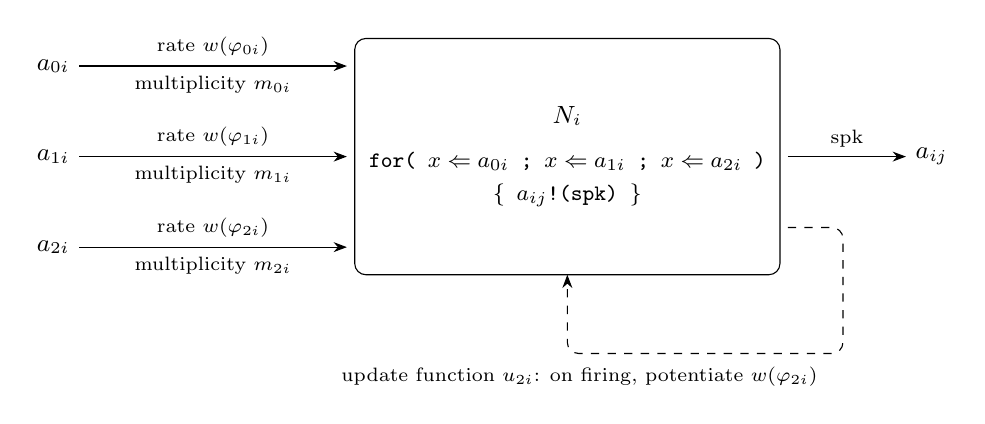
\begin{tikzpicture}[>=Stealth]
  \node[draw, rounded corners, minimum width=54mm, minimum height=30mm, align=center] (N) at (0,0)
    {\small $N_i$\\[4pt]
     \footnotesize\ttfamily for( $x\Leftarrow a_{0i}$ ; $x\Leftarrow a_{1i}$ ; $x\Leftarrow a_{2i}$ )\\
     \footnotesize\ttfamily \{\ $a_{ij}$!(spk)\ \}};
  \foreach \k/\y in {0/1.15, 1/0.0, 2/-1.15} {
    \node[anchor=east] (d\k) at (-6.2,\y) {\small $a_{\k i}$};
    \draw[->] (d\k.east) -- node[above, font=\scriptsize, pos=0.5] {rate $\wmap(\varphi_{\k i})$}
              node[below, font=\scriptsize, pos=0.5] {multiplicity $m_{\k i}$} (-2.8,\y);
  }
  \node[anchor=west] (o) at (4.3,0) {\small $a_{ij}$};
  \draw[->] (2.8,0) -- node[above, font=\scriptsize] {spk} (o.west);
  \draw[->, dashed, rounded corners]
    (2.8,-0.9) -- (3.5,-0.9) -- (3.5,-2.5) -- (0,-2.5) -- (0,-1.5);
  \node[font=\scriptsize, anchor=north east] at (3.3,-2.55)
    {update function $u_{2i}$: on firing, potentiate $\wmap(\varphi_{2i})$};
\end{tikzpicture}
\caption{A neuron. The three factors of Definition~\ref{def:propensity} are visible: the weight map
supplies a rate constant per synapse, the marking supplies multiplicity, and the geometric factor is
$1$. The dashed arrow is the refinement entry's update function, which is where plasticity lives.}
\label{fig:neuron}
\end{figure}

\subsection{The keys, and why they form a partition}

\begin{definition}[Synaptic keys]
\label{def:synkeys}
For each synapse $(j,i)$ put
\[
\varphi_{ji} \;\;\triangleq\;\; \inn(a_{ji})\top \;\sepc\; \out(a_{ji})\top ,
\]
the formula holding of a communication redex on $a_{ji}$, and let
$\Phi_{\textsc{comm}} = \{\varphi_{ji}\} \cup \{\varphi_\bot\}$ with
$\varphi_\bot = L^\sharp \wedge \neg\bigvee_{ji}\varphi_{ji}$.
\end{definition}

\begin{proposition}
\label{prop:rnn-admissible}
$\Phi_{\textsc{comm}}$ is admissible, with $\alpha = 2$.
\end{proposition}

\begin{proof}
Distinct synapses are distinct channels, and a communication redex is on exactly one channel, so
(P1) holds; $\varphi_\bot$ gives (P2) by Remark~\ref{rem:default}. Each key has depth $2$ by
Definition~\ref{def:depth}, and checking $\inn(a)\top \sepc \out(a)\top$ against a term is a bag
lookup, so \ref{req:dec} and \ref{req:loc} hold.
\end{proof}

The weight $\wmap(\varphi_{ji})$ is the efficacy of synapse $(j,i)$. Nothing else in the presentation
mentions it.

\subsection{Threshold is join structure}

\begin{proposition}[McCulloch--Pitts, as an expressivity lemma]
\label{prop:mcp}
The threshold presentation of Definition~\ref{def:neuron} realises the monotone Boolean threshold
function $\mathbf{1}[\,\sum_{j} \mathbf{1}[a_{ji}\text{ populated}] \geq \theta_i\,]$: the neuron has
an enabled redex exactly when at least $\theta_i$ of its dendrites carry a pending spike. It uses
$\binom{k_i}{\theta_i}$ join groups.
\end{proposition}

\begin{proof}
A group $S$ is enabled iff every $a_{si}$ for $s \in S$ carries a spike, since $\&$ requires
simultaneous availability of all its binds; the receipt is enabled iff some group is, since $;$
separates alternatives. Some $\theta_i$-subset is fully populated iff at least $\theta_i$ dendrites
are populated. The count of groups is the count of $\theta_i$-subsets.
\end{proof}

So the historical origin of the neuron model --- McCulloch and Pitts' threshold unit \cite{mcp} ---
is not encoded in a weighted GSLT but \emph{is} a for-comprehension, with the threshold appearing as
the arity of the joins and the alternatives as the group separator. We now state this as an
expressivity lemma and not, as the first version implied, as a practical construction, and the
qualification is not cosmetic. $\binom{k}{\theta}$ groups is unusable at realistic fan-in, so the
scalable presentation is the one at $\theta = 1$, where threshold behaviour is trivial and the join
structure carries no weight. What the lemma establishes is that no apparatus beyond the
for-comprehension is needed to \emph{express} a threshold; what it does not establish is that this is
how one would build a large network.

\begin{remark}[The combinatorial blowup, and the \texttt{where} clause]
Rholang~1.4's for-comprehension carries a \texttt{where} clause \cite{omnibus}, which collapses the
presentation to a single group at the cost of changing the semantics: \texttt{for($x_1 \Leftarrow
a_{1i}\ \&\ \cdots\ \&\ x_k \Leftarrow a_{ki}$ where $\phi$)} waits for \emph{all} $k$ dendrites and
then gates on $\phi$. That is a coincidence detector with a filter, not a threshold unit. The two
presentations agree at $\theta = k$ and differ elsewhere, and which one a modeller wants is a
modelling question. We use $\theta_i = 1$ below, where both are trivial and the group presentation
has $k_i$ single-bind alternatives.
\end{remark}

\begin{remark}[Coincidence versus rate]
$\theta_i = k_i$ gives a pure coincidence detector: the neuron fires only on simultaneous arrival at
every dendrite. $\theta_i = 1$ gives a pure rate integrator: any arrival can trigger it, and the
weights determine how fast. Real cortical neurons sit between, and so does the presentation, with
$\theta$ as the dial. This is a rare case in which a biological parameter and a syntactic parameter
are the same parameter.
\end{remark}

\subsection{The weighted sum, and where the squashing function went}
\label{sec:squash}

Take $\theta_i = 1$, so $N_i$ has $k_i$ single-bind alternatives, and let the marking assign $m_{ji}$
pending spikes to dendrite $a_{ji}$.

\begin{proposition}[Propensity of a neuron]
\label{prop:neuron-prop}
With $\gfac \equiv 1$ and $\chi \equiv 1$, the total propensity of the redexes belonging to neuron
$i$ is
\[
\prop_i \;=\; \sum_{j} \wmap(\varphi_{ji}) \cdot m_{ji} .
\]
\end{proposition}

\begin{proof}
The receipt is persistent, so exactly one input is available on each $a_{ji}$, and the marking
supplies $m_{ji}$ outputs; by Definition~\ref{def:redex} the number of redexes classified
$\varphi_{ji}$ is $1 \cdot m_{ji}$. Definition~\ref{def:propensity} gives $\wmap(\varphi_{ji})m_{ji}$
per synapse, and the classes are disjoint by Proposition~\ref{prop:rnn-admissible}, so
Proposition~\ref{prop:total} lets them be summed.
\end{proof}

Formally this is the weighted sum $\sum_j w_{ji} m_{ji}$ of the textbook artificial neuron, with the
presynaptic activity $m_{ji}$ read as the marking, and it has not been written into any term; it is
what Definition~\ref{def:propensity} computes. The comparison should nevertheless be made carefully,
because the two quantities are not the same kind of thing. $\prop_i$ is a hazard rate, with units of
inverse time, governing a race between exponential clocks. It is not an affine pre-activation waiting
to be passed through an activation function, and the first version of this note wrote as though it
were. What the next corollary shows is that a saturating nonlinearity nevertheless appears, and
appears without being supplied.

\begin{corollary}[The response saturates and nobody wrote it]
\label{cor:sigmoid}
Hold the marking on $i$'s dendrites fixed over a window $[0,\Delta]$. The probability that neuron $i$
fires at least once in the window is
\[
\Pr[\,\text{$i$ fires}\,] \;=\; 1 - \exp\!\big(-\Delta \textstyle\sum_j \wmap(\varphi_{ji}) m_{ji}\big),
\]
a monotone function of the weighted sum, with slope $\Delta$ at the origin and asymptote $1$.
\end{corollary}

\begin{proof}
Under a marking held fixed on $i$'s dendrites the propensity $\prop_i$ is constant, so firings of $i$
within the window are the events of a homogeneous Poisson process of rate $\prop_i$, by
Theorem~\ref{thm:markov} restricted to the sub-chain along which $m_{\cdot i}$ does not change. The
probability of at least one event in $[0,\Delta]$ is $1 - e^{-\prop_i \Delta}$.
\end{proof}

Two provisos, one standard and one easy to miss.

The standard one is that the marking is not in fact frozen, since other neurons are firing into it.
Corollary~\ref{cor:sigmoid} is a statement about a window short enough that the input has not moved,
which is the usual justification for a rate-coded neuron and the usual approximation.

The one that is easy to miss --- and that the first version's proof did miss, freezing only the other
neurons --- is that $i$'s own firings change the marking. A firing consumes a spike from the dendrite
it fired on, so $\prop_i$ drops and the process is not homogeneous past the first event unless the
marking is externally replenished. The hypothesis must therefore be read as freezing $m_{\cdot i}$
against \emph{all} sources of change, $i$'s own consumption included. That is exactly the
standing-input regime in which a rate code is normally discussed, and it is why the statement is
about the first event rather than about a count.

\begin{remark}[Saturating, not logistic]
\label{rem:not-logistic}
$1 - e^{-\Delta x}$ is an exponential saturation function. It is not the logistic
$\sigma(x) = (1+e^{-x})^{-1}$, and the first version of this note said that it was --- in this
section, and in its abstract, where the emergence of a logistic response was offered as a selling
point. The correct claim is worth as much and should be stated exactly: \emph{a saturating nonlinear
activation emerges from exponential race semantics without being programmed into the term}. No
squashing function was supplied and none is needed. A neuron under enormous drive still cannot fire
more than once per event, so its firing probability per window is bounded by $1$ however large the
weighted sum grows, and that bound is the waiting-time law of the chain rather than a modelling
choice.
\end{remark}

\subsection{Boundedness}
\label{sec:rnn-bounded}

\begin{lemma}[Boundedness]
\label{lem:bounded}
Let $f_i = |\mathrm{post}(i)|$ be the fan-out of neuron $i$. If $f_i \leq \theta_i$ for every $i$,
the total number of pending spikes is non-increasing along every run, the reachable term set is
finite, and $\mathsf{Net}$ is term-finite in the sense of Definition~\ref{def:bounded}.
\end{lemma}

\begin{proof}
Firing $N_i$ consumes $\theta_i$ pending spikes (one per bind in the selected group) and produces
$f_i$. The total marking therefore changes by $f_i - \theta_i \leq 0$. Since the neurons are
persistent and the channel set is fixed, a term reachable from $\mathsf{Net}$ is determined by its
marking, and markings with at most $|M_0|$ tokens over finitely many channels are finite in number.
\end{proof}

The hypothesis is restrictive: it forbids fan-out exceeding threshold, which most networks want. Two
standard repairs, both expressible in the theory:

\begin{enumerate}[leftmargin=2.2em]
\item \emph{Capacity.} Guard the neuron body's sends by a \texttt{where} clause bounding the
occupancy of the target channel \emph{after} the firing by $c$. The marking is then bounded by $c$
per channel and the state space by $c^{|\vec a|}$, restoring term-finiteness unconditionally. This is
a saturating synapse, and it is what a real one does. The post-firing reading is not fussiness: the
obvious alternative, refusing a send when the target is already full, blocks the consumer and
deadlocks the network (\S\ref{sec:built}).
\item \emph{Leak.} Add a base rule $a_{ji}!(\mathrm{spk}) \leadsto \Nil$ with its own key and weight
$\lambda_{\text{leak}}$. This does not restore term-finiteness by itself but makes the marking
positive-recurrent, which is enough for the stationary analysis and for classical simulation, though
not for \S\ref{sec:quantum}.
\end{enumerate}

We take capacity in what follows, since \S\ref{sec:rnn-quantum} needs a finite-dimensional
$\mathcal{H}$.

\begin{remark}[The network is a marked graph]
Under Lemma~\ref{lem:bounded}, $\mathsf{Net}$ is a live, bounded, conservative marked graph in the
Petri-net sense, and the analysis of \cite{knots} applies verbatim: a \emph{period} is a firing
schedule returning the marking to its initial value, and it is the right analogue of a timestep. The
weighted-GSLT layer adds what a marked graph does not have, namely a probability distribution over
which of the enabled transitions fires next and how long it takes.
\end{remark}

\subsection{Plasticity is the update function}
\label{sec:plasticity}

\begin{definition}[Local potentiation entry]
\label{def:hebb}
Equip the communication rule's entry at $\varphi_{ji}$ with
\[
u_{ji}(\wmap) \;=\; \wmap\big[\,\varphi_{ji} \mapsto \min\{\,w_{\max},\ \wmap(\varphi_{ji}) + \eta\,\}\,\big],
\]
for a potentiation increment $\eta > 0$ and ceiling $w_{\max}$. The ceiling is not cosmetic: with a
quantised increment it is what makes the reachable weight-map set finite, which
Remark~\ref{rem:map-finite} requires of \S\ref{sec:rnn-quantum}.
\end{definition}

So the augmented rule reads, in full:
\begin{center}
\begin{minipage}{0.92\textwidth}
\begin{lstlisting}
COMM . |- (PPar {(PForUser rows p), (POutput n q), ...rest})
        ~> (PPar {(subst ...), ...rest})  [1.0] {
      phi(0,1) => (w_01, hebb(0,1)),
      phi(1,1) => (w_11, hebb(1,1)),
      ...
      phi_bot  => (0.0,  id)
   };
ParCong . | S ~> T |- (PPar {S, ...rest}) ~> (PPar {T, ...rest})  [1.0] { snd };
\end{lstlisting}
\end{minipage}
\end{center}

\begin{theorem}[Learning and inference are one relation]
\label{thm:one-relation}
Let $\mathsf{Net}$ be a weighted GSLT as above. The transition relation of
Definition~\ref{def:transition} on $\Cfg = \Terms \times \Wt$ has two marginals: the projection to
$\Terms$ is the network's inference dynamics, and the projection to $\Wt$ is its learning dynamics.
Neither is a separate process. In particular there is no training schedule, no separate learning
clock, and no distinguished learning phase; the learning rate $\eta$ is not a hyperparameter of an
outer loop but a component of the theory, sitting in the same refinement entry as the weight it
modifies.
\end{theorem}

\begin{proof}
Immediate from Definitions~\ref{def:config} and \ref{def:transition}: a single step produces
$(P', \wmap')$ with $P'$ obtained by the rewrite and $\wmap'$ by the fold of the update function.
\end{proof}

This is the claim the example exists to make, and it is exactly what a static-rate calculus cannot
express. In SPiM a rate is fixed at declaration, so a stochastic $\pi$ model of a neural network can
model the firing but not the learning; one must step outside the calculus, adjust the rates, and
re-run. Here the adjustment is a transition of the same system.

\begin{remark}[How Hebbian this is]
\label{rem:hebbian}
Definition~\ref{def:hebb} potentiates $\varphi_{ji}$ when a communication on $a_{ji}$ fires --- that
is, when a presynaptic spike is consumed by an enabled postsynaptic receipt. The event is local and
activity-dependent, and the condition ``pre and post were jointly involved'' is not a correlation
computed by an observer but the firing of a single rewrite, which by construction requires both
parties. That much is the structural content of Hebb's proposal \cite{hebb} and it is the part worth
having: the event which transmits is the event which potentiates, because a communication is one
rewrite.

It is nevertheless less than Hebbian learning as usually meant, and the first version of this note
was too generous in saying that cells which fire together wire together \emph{literally}. Hebbian
plasticity invokes a correlation between pre- and \emph{postsynaptic firing}; successful transmission
into an enabled receipt is not by itself postsynaptic firing, since the receiving neuron may not
reach threshold. What Definition~\ref{def:hebb} gives is a minimal local Hebbian potentiation rule,
and \S\ref{sec:stdp} says what the timing-dependent version costs.
\end{remark}

\subsection{Spike-timing dependence needs a wider update signature}
\label{sec:stdp}

Spike-timing-dependent plasticity makes $\Delta w$ a function of the interval between pre- and
postsynaptic spikes, potentiating for pre-before-post and depressing for the reverse \cite{stdp}.
The ingredients are available --- the simulator of Definition~\ref{def:ssa} produces a timestamp at
every step --- but the update function of Definition~\ref{def:augmented} cannot see them, since its
type is $\Wt \to \Wt$.

\begin{definition}[Extended update]
\label{def:extended-update}
Replace $u_i : \Wt \to \Wt$ by
\[
u_i \;:\; \Wt \times \mathrm{Match} \times \partial\Terms \times \mathbb{R}_{\geq 0} \times \mathcal{S} \longrightarrow \Wt ,
\]
taking additionally the matched substitution $\sigma$, the position $k$ at which the rule fired, the
current simulation time $t$, and a bounded \emph{trace summary} $\mathcal{S}$ --- for STDP, one
eligibility trace per synapse, itself decaying at a rate specified in the theory.
\end{definition}

Theorem~\ref{thm:markov} survives this extension provided $\mathcal{S}$ is finite-dimensional and
updated deterministically, since one simply enlarges the configuration to
$(P, \wmap, \mathcal{S})$; it does \emph{not} survive an update function reading unbounded history,
which would make the process genuinely non-Markovian and put exact simulation out of reach. The
eligibility-trace formulation of STDP is precisely the standard device for staying inside the
bounded case, and it is pleasant that the constraint arrives here from the requirement that the
chain be a chain rather than from computational convenience.

\subsection{Uniformity: one theory for every network}
\label{sec:rnn-uniform}

Definition~\ref{def:synkeys} gives one key per synapse, so a network with $10^4$ synapses has $10^4$
keys and a network that grows needs a new theory. Reflection removes both problems. Following the
construction of \cite{knots}, take the synapse channels to be structured names
\[
a_{ji} \;=\; @[\,*\mathit{net},\, j,\, i\,],
\]
so that a name predicate can recover the endpoints. Then
\[
\varphi_{\mathrm{syn}} \;\triangleq\; \exists j, i.\; \inn(@[*\mathit{net},j,i])\top \;\sepc\; \out(@[*\mathit{net},j,i])\top
\]
is a single key describing the whole \emph{namespace} of synapses of this network, which is
namespace logic doing what it was built for \cite{namespace}. The weight map then has one entry per
network rather than per synapse; per-synapse efficacies are recovered by letting the entry's value be
a function of the recovered indices, which is the standard move of trading a large map for a small
map with structured keys. A greatest fixed point makes ``every neuron reachable from $i$ eventually
fires'' a single formula rather than an $n$-fold conjunction, which is the uniformity $\nu$ buys
\cite[\S3]{classifier}. In an atomic-name calculus none of this is available: the indices would have
to travel as message payloads and the logic could reach them only by observing traffic.

\subsection{The quantum network}
\label{sec:rnn-quantum}

Replace the efficacies by amplitudes $z_{ji} \in \Cx$, with $\lambda(z_{ji}) = |z_{ji}|^2$ the rate
each denotes and no bound on the modulus (Remark~\ref{rem:rnn}), keeping the keys, the neurons and
the capacity bound. Definition~\ref{def:jump} gives a jump operator per synapse,
Definition~\ref{def:qctmc} a Lindbladian, and Definition~\ref{def:qjump} a trajectory simulator.

The example satisfies the hypothesis of Definition~\ref{def:hilbert} in both components, which is why
it is the example: the capacity bound of \S\ref{sec:rnn-bounded} makes the reachable term set finite,
and the ceiling $w_{\max}$ of Definition~\ref{def:hebb}, with a quantised increment, makes the
reachable map set finite. So $\mathcal{H}$ is finite-dimensional over \emph{configurations}, the
model checking of \cite{qctmc,qctmc-csl} applies, and the projectors come from
Proposition~\ref{prop:projective}: $\Pi_{\varphi_{\mathrm{syn}}}$, for instance, has expectation the
probability that the network has an available synaptic transmission at time $t$.

\begin{remark}[Indistinguishable spikes do not interfere]
\label{rem:bosonic}
By Remark~\ref{rem:distinct-contracta}, $m$ indistinguishable pending spikes on $a_{ji}$ give $m$
redexes with a common contractum, and a reader of the first version of this note will recall the
claim that the quantum network is therefore superlinear in presynaptic multiplicity, transmitting at
$m^2|z_{ji}|^2$ where the classical network transmits at $m|z_{ji}|^2$.
Proposition~\ref{prop:bosonic} withdraws it. Under the normalisation of Definition~\ref{def:jump} the
amplitude of the synaptic jump channel is $\sqrt{m}\,|z_{ji}|$, its weight is $m|z_{ji}|^2$, and at
$H = 0$ the quantum network's population dynamics is exactly the classical network's.

What the complex reading adds to \S\ref{sec:rnn} is therefore not an enhancement of transmission but
a coherent channel between configurations that the equational presentation declines to quotient ---
and the presentation of Definition~\ref{def:neuron} quotients everything, so as written it adds
nothing at all. This is a sharper and less flattering statement than the first version's, and it has
the merit of naming what would have to be done: constructing a spiking network whose equational
theory leaves something coherent, so that Definition~\ref{def:hamiltonian} has material to work with.
We have not done it, and we no longer claim that concurrency supplies it for free.
\end{remark}

\subsection{What this example does not show}

Honesty about scope. The learning here is local and Hebbian; nothing above implements
backpropagation, which needs a global error signal propagated against the direction of inference.
One can encode such a signal as traffic on a second family of channels with its own keys, and the
apparatus does not forbid it, but the result would no longer have the property that makes
Theorem~\ref{thm:one-relation} interesting --- the error channel is an outer loop wearing a costume.
Whether a genuinely local weighted-GSLT learning rule can match backpropagation is not a question
this note answers, and the honest statement is that the example demonstrates a \emph{mechanism} for
plasticity inside the calculus, not a competitive learning algorithm.

Nor do we claim biological fidelity. The neuron of Definition~\ref{def:neuron} has no membrane
potential, no refractory period, and no dendritic geometry. The first two are easy additions --- a
potential is a payload, a refractory period is a guard --- and the third is what the geometric factor
$\gfac$ of \S\ref{sec:geometric} is for, which is a use we have not developed.

\section{Implementation}
\label{sec:impl}

\subsection{Surface syntax}
\label{sec:surface}

The weighting is a decoration of MeTTaIL's \texttt{rewrites} block, and it should read as one. The
existing surface is
\begin{center}
\begin{minipage}{0.88\textwidth}
\begin{lstlisting}
rewrites {
    Exec    . |- (PDrop (NQuote P)) ~> P;
    ParCong . | S ~> T |- (PPar {S, ...rest}) ~> (PPar {T, ...rest});
}
\end{lstlisting}
\end{minipage}
\end{center}
and the weighted surface adds a bracketed weight and a brace block after the rule, in both cases
optional:
\begin{center}
\begin{minipage}{0.88\textwidth}
\begin{lstlisting}
rewrites {
    // base rule: [scalar] { key => (weight, update) }
    COMM . |- (PPar {(PForUser rows p), (POutput n q), ...rest})
            ~> (PPar {(subst rows p q), ...rest})   [1.0] {
        in(n)TOP | out(n)@fast  => (2.5, scale(0.9)),
        in(n)TOP | out(n)TOP    => (0.7, id),
        default                 => (0.0, id)
    };

    // base rule, unweighted: defaults to [1.0] { default => (1.0, id) }
    Exec . |- (PDrop (NQuote P)) ~> P;

    // context rule: [geometric factor] { fold }
    ParCong . | S ~> T |- (PPar {S, ...rest}) ~> (PPar {T, ...rest})  [1.0] { snd };
}
\end{lstlisting}
\end{minipage}
\end{center}

Notes on the design. \texttt{default} is sugar for the completion of
Remark~\ref{rem:default} --- the elaborator synthesises
$L^\sharp \wedge \neg\bigvee_i \varphi_i$ --- so a modeller writes exclusive keys and gets a
partition. Exclusivity itself is checked at elaboration time and is a hard error, not a warning,
since Proposition~\ref{prop:classify} fails without it. Keys are written in the concrete syntax of
the generated logic; the two shown are ordered from more to less specific purely for readability,
since exclusivity means order is semantically irrelevant. A context rule's default factor is
$1$ and its default fold is \texttt{snd}, which together implement ``addressing is free and does not
touch the map'' (\S\ref{sec:geometric}).

\subsection{What is built}
\label{sec:built}

The first version of this note measured itself against a prototype called \texttt{mettail-gillespie},
whose \texttt{TermRef} was an opaque identifier, whose spatial behaviours were a hand-rolled enum,
whose rates were clamped to the unit interval, and whose quantum module was amplitude bookkeeping
over a classical branching structure. That crate no longer exists. It has been superseded by
\texttt{rho-weighted} \cite{gillespie-crate}, and the report is now close to the opposite of the one
it replaces: the implementation is ahead of the first version's specification on every point that
version listed as a gap, and in the course of being built it found three errors in the specification
itself.

\paragraph{What the crate is.} A \emph{simulator}, and deliberately not the interpreter. The
interpreter maintains the state of a running shard; the simulator answers what would happen if,
across a family of hypothetical configurations, and yields transition graphs, generators and
parameter sweeps rather than a single history. That separation is what makes exhaustive graph
construction, greatest fixed points and the whole of \S\ref{sec:quantum} affordable here and
unaffordable there, and it is why the crate owns its own space --- an immutable channel index with
cheap forking --- rather than a tuple space with checkpoints. It shares the interpreter's matching
semantics without sharing its code paths, which makes agreement between them an obligation rather
than a theorem; see below.

\paragraph{Correspondence with this note.}
\begin{center}
\begin{tabular}{@{}ll@{}}
\toprule
Specification & Implementation \\
\midrule
Definitions \ref{def:partition}--\ref{def:reqs}, admissibility & partition and fragment checks; failure is an error, never a fallback \\
Proposition~\ref{prop:classify}, classification & the classifier, total by construction \\
Definition~\ref{def:propensity}, propensity & organised by redex, per Proposition~\ref{prop:total} \\
Definition~\ref{def:ssa}, the SSA & the sampler, with provenance recorded per run \\
Theorem~\ref{thm:markov}, the generator & exhaustive graph plus $Q$, diagonal per Remark~\ref{rem:selfloop} \\
Definition~\ref{def:extended-update}, updates & the update context: bindings, position, clock, trace \\
\S\ref{sec:rnn}, the network & the worked example, end to end \\
Definitions \ref{def:jump}--\ref{def:qjump}, the quantum path & density operators, $\Heff$, unravelling \\
\bottomrule
\end{tabular}
\end{center}

\paragraph{Three corrections the implementation made to the specification.} These are the reason this
section is worth reading rather than a table of ticks.

\begin{enumerate}[leftmargin=2.2em]
\item \emph{Multiplicity is invisible in a trace.} The superseded prototype omitted the cardinality
of $K(r,\varphi,P)$ entirely, and its traces looked entirely plausible; nothing an eye could catch
distinguishes a chain running at the wrong rate from one running at the right rate. Acceptance
therefore has to be statistical rather than observational. The birth--death theory is checked against
a truncated Poisson law, with a control asserting that the Poisson and geometric laws are half a unit
of total variation apart, so that the test cannot pass vacuously against a chain that ignores
multiplicity.
\item \emph{A capacity guard must be evaluated post-firing.} The obvious reading of the guard of
\S\ref{sec:rnn-bounded} --- refuse a send when the target channel is already at capacity --- blocks
the consumer and deadlocks the network. The guard must bound occupancy \emph{after} the firing it
gates. Relatedly, a hard capacity makes a token amplifier absorbing rather than live, which is a stop
and not a deadlock; a network that is to saturate and keep running wants the leak rule of
\S\ref{sec:rnn-bounded} instead, trading term-finiteness for positive recurrence and thereby giving
up \S\ref{sec:quantum}.
\item \emph{Remark~\ref{rem:scalar-damping}.} The claim that a nonzero Hamiltonian suffices for a
non-exponential sojourn is false under uniform exit rates. The test that separates the two cases is
what found it.
\end{enumerate}

\paragraph{What is outstanding.} Three items, and they are not the ones the first version listed.
\begin{enumerate}[leftmargin=2.2em]
\item \emph{The logic is hand-written, not generated.} The connectives of \S\ref{sec:logic} are
implemented by hand behind a port whose interface is the one an OSLF-generated instance would
implement, so the swap is at the boundary rather than through the simulator, which was the design
intent. Until it lands, the genericity over GSLTs claimed in \S\ref{sec:intro} is argued and not
demonstrated, and that is the largest gap in the note.
\item \emph{Surface syntax.} \S\ref{sec:surface} is a design and not a grammar. It needs parser and
tree-sitter changes in a separate repository on a separate release cadence; theories are built
programmatically today, and nothing else in the crate depends on the syntax landing.
\item \emph{Faithfulness.} Because the simulator and the interpreter share semantics but not code
paths, their agreement is a permanent obligation. What runs today is a differential against an
independently written reference matcher over a corpus of several hundred cases, together with a
negative control establishing that the corpus can detect a broken matcher. The differential against
the interpreter's own matcher is written, is gated behind a build feature, and has not been run,
because the workspace it needs does not currently build from a clean checkout. The gap is visible in
the test output by design rather than recorded only here.
\end{enumerate}

\paragraph{Two known incompletenesses.} First, the partition check evaluates (P1) and (P2) against a
supplied set of witnesses. It is therefore a sound \emph{refuter} --- an overlap it reports is real
--- and not a proof of admissibility, which would require deciding entailment in the generated logic.
By Observation~\ref{obs:closure} this is exactly the price of taking the external branch, and it
should be read as such rather than as a deficiency of the check. Second, the checkable-fragment gate
currently admits modal and fixed-point formulae as keys, which \ref{req:str} forbids; enforcing
\ref{req:str} at elaboration time is a small change and is the precondition for the incremental
scheme below.

\subsection{Incremental propensity}
\label{sec:incremental}

Lemma~\ref{lem:locality} licenses the standard optimisation. Maintain $\prop$ as a Fenwick tree over
$(r,\varphi)$ classes with per-class redex lists; after firing at position $k$, reclassify only
redexes within radius $\alpha + |L| + |R|$ of $k$, and additionally rescale the classes whose weight
the update function touched --- which for Definition~\ref{def:hebb} is exactly one class. The second
part is the only respect in which dynamic weight maps cost anything at run time, and it is cheap
precisely when update functions are sparse. A modeller who writes an update function touching every
entry pays a full recomputation of $\prop_0$ per step, and should be told so.

\section{Weights and costs}
\label{sec:cost}

Cost accounting and weighting both decorate rewrites, and it is worth stating plainly that they are
different decorations doing different jobs.

A cost decoration attaches to a rewrite a debit against a token stack, and the funding judgment
$\Sigma \funds \Delta$ --- decidable, total, monotone in supply --- decides whether a step may occur
at all \cite{costmonad}. It is implemented in the transpiler branch as
\texttt{OslfResourceLogic}, with a supply multiset keyed by signature and a demand list, one token
per signed term, and conformance laws asserting soundness, rejection of underfunding, supply
monotonicity, and decidability. A weight decoration attaches a rate, and decides how fast and how
often. The composition is one-directional:

\begin{definition}[Funding gate]
\label{def:gate}
For a redex $(k,\sigma)$ of rule $r$, let $\Delta(r,k,\sigma)$ be the demand it incurs and
$\Sigma(P,k)$ the supply available at that location. Put
$\chi(r,k,\sigma) = 1$ if $\Sigma(P,k) \funds \Delta(r,k,\sigma)$ and $0$ otherwise.
\end{definition}

\begin{proposition}[Cost gates the support, weight distributes over it]
\label{prop:gate}
With $\chi$ as in Definition~\ref{def:gate}, the coalgebra of Definition~\ref{def:coalgebra}
restricts to the funded sub-transition-system: unfunded redexes have propensity zero and contribute
nothing to $\prop_0$, while among funded redexes the distribution is unchanged from the
cost-free case up to normalisation.
\end{proposition}

\begin{proof}
$\chi$ appears as a multiplicative factor in Definition~\ref{def:propensity}, taking values in
$\{0,1\}$; a zero factor removes the term from the sum, and the remaining terms are untouched.
\end{proof}

Three consequences worth recording.

\emph{The gate is decidable, so the simulator stays exact.} If funding were a real-valued penalty
rather than a Boolean, the propensity would depend on an optimisation and the chain would no longer
be simulable by Definition~\ref{def:ssa}. The decidability law of the resource logic is doing real
work here.

\emph{Exhaustion is a halting condition, not a deadlock.} $\prop_0 = 0$ when every enabled redex is
unfunded, and Definition~\ref{def:ssa} halts. The chain has reached an absorbing state, which is the
correct reading: a system that cannot pay for any of its available transitions has stopped, and the
waiting time to the next event is infinite rather than undefined.

\emph{The neural example acquires a metabolism.} Give the communication rule a phlogiston demand per
firing and the network of \S\ref{sec:rnn} has an energy budget: a neuron whose local supply is
exhausted has propensity zero regardless of its synaptic weights, and the network's activity is
bounded by its funding rather than by its capacity guard. Weight is what a synapse is worth; cost is
what a spike costs. Separating them is what lets a model say that a strong synapse on a starving
neuron is silent, which is a statement neither decoration makes alone. This is the point of contact
with the mortal-computation reading of \cite{scientist}, and we go no further with it here.

\section{Open threads}
\label{sec:open}

\begin{enumerate}[leftmargin=2.2em]
\item \emph{A combined logic.} \S\ref{sec:qctmc-logic} has the generated logic supplying projectors
to an external temporal logic. What one wants is a single logic with context-labelled modalities and
time-bounded operators --- $\langle K_j \rangle^{\leq t}\varphi$ --- adequate for weighted
bisimulation on configurations. The classical half of this is well trodden (CSL over CTMCs); the
question is what OSLF emits when the presentation it is fed is already weighted.
\item \emph{Weighted bisimulation.} The category \textbf{GSLT} has bisimulation-preserving maps as
morphisms \cite{omnibus}. What is the right notion when the objects carry weight maps? Rate
bisimulation (lumpability) is the obvious candidate for $\Rnn$, and since \S\ref{sec:bosonic} makes
the complex case conservative over the real one, the same candidate transfers to the populations of
$(\mathcal{H},\mathcal{L})$ at $H = 0$ without further work. The open case is $H \neq 0$, where a
relation on configurations must also respect coherences, and where we have no candidate.
\item \emph{Per-derivation amplitudes.} \S\ref{sec:bosonic} fixes the normalisation of a jump channel
by conservativity, and the price is that no coherence arises from the rewrite relation at all.
Rewrite-level interference would require amplitudes attached to \emph{derivations} rather than to
refinement classes --- a weight map whose domain is $\coprod_r \Phi_r \times \partial\Terms$, or some
quotient of it, so that two routes to a common contractum can carry different phases. Whether such a
decoration can be given without destroying Lemma~\ref{lem:locality} and without making the map's size
grow with the term is the question. Note that this is a strictly larger construction and not a repair
of the present one, which is complete and conservative as it stands.
\item \emph{Geometric factors.} \S\ref{sec:geometric} identifies $\gfac$ as the natural home of a
spatial weighting and declines to develop it. The gravitation correspondence of
\cite{costspacetime} splits a weight on a reduction-graph edge into a geometric part and a matter
part; here $\gfac(k)$ is visibly the first and $\wmap(\varphi)$ visibly the second, and the
correspondence asks for an action forcing the two to agree. That is a paper.
\item \emph{Quantale weights.} A quantale-valued codomain gives a fuzzy calculus, and \cite{fuzzy}
develops the flat-substitution instance independently. Whether it is an instance of
Definition~\ref{def:wmap} or a genuinely different decoration --- the fuzzy comm rule transmits a
modified payload, which no weighting here does --- is not settled. Remark~\ref{rem:codomain} sharpens
the test: a codomain is a genuine instance of the parameter only if it comes with an interpretation
map into $\Rnn$ under which the propensity of Definition~\ref{def:propensity} is unchanged, and the
interesting question about the quantale case is whether it has one.
\item \emph{Map-finiteness as a hypothesis.} Remark~\ref{rem:map-finite} makes finiteness of the
reachable weight-map set a requirement of \S\ref{sec:quantum} rather than a caveat, so quantised or
saturated weights are mandatory there. Quantised weights make $\Cfg$ finite and the whole apparatus
model-checkable; they also make the learning dynamics a finite automaton, whose reachable weight
configurations are an object nobody has looked at.
\item \emph{Locality for modal keys.} \ref{req:str} excludes behavioural modalities from keys because
Lemma~\ref{lem:locality} fails for them, and a rate that depends on what a redex can do next is a
natural thing for a modeller to want. The question is whether a bounded-lookahead modality
$\langle K\rangle^{\le n}$ admits a locality lemma with radius depending on $n$, or whether modal keys
simply cost global reclassification at every step. The second is what an implementation must assume
until the first is proved.
\end{enumerate}

\begin{thebibliography}{99}

\bibitem{classifier} L.\ G.\ Meredith. \emph{Classifying knots with spatial--behavioural logics.}
F1R3FLY.io working note, 2026.

\bibitem{costmonad} L.\ G.\ Meredith. \emph{Cost accounting as an endofunctor on continued
interactive GSLTs.} F1R3FLY.io working note, 2026.

\bibitem{costspacetime} L.\ G.\ Meredith. \emph{Cost, spacetime, and the geometry/matter split on
reduction graphs.} F1R3FLY.io working notes, 2026.

\bibitem{dalibard} J.\ Dalibard, Y.\ Castin and K.\ M\o lmer. Wave-function approach to dissipative
processes in quantum optics. \emph{Physical Review Letters} 68(5):580--583, 1992.

\bibitem{fuzzy} \emph{Fuzzy rho-calculus: a quantale-graded interaction, and its lift to ciGSLTs with
binding.} F1R3FLY.io working note, 2026.

\bibitem{gibson-bruck} M.\ A.\ Gibson and J.\ Bruck. Efficient exact stochastic simulation of
chemical systems with many species and many channels. \emph{Journal of Physical Chemistry A}
104(9):1876--1889, 2000.

\bibitem{gillespie77} D.\ T.\ Gillespie. Exact stochastic simulation of coupled chemical reactions.
\emph{Journal of Physical Chemistry} 81(25):2340--2361, 1977.

\bibitem{gillespie-crate} F1R3FLY.io. \texttt{mettail-gillespie}: stochastic and quantum Gillespie
simulation extensions for MeTTaIL rewrite rules. \texttt{F1R3FLY-io/publications},
\texttt{rho-life/Gillespie}, 2026.

\bibitem{hebb} D.\ O.\ Hebb. \emph{The Organization of Behavior.} Wiley, 1949.

\bibitem{knots} L.\ G.\ Meredith. \emph{Knots as cost-accounted processes.} F1R3FLY.io working note,
2026.

\bibitem{mcp} W.\ S.\ McCulloch and W.\ Pitts. A logical calculus of the ideas immanent in nervous
activity. \emph{Bulletin of Mathematical Biophysics} 5:115--133, 1943.

\bibitem{mcwf} K.\ M\o lmer, Y.\ Castin and J.\ Dalibard. Monte Carlo wave-function method in quantum
optics. \emph{Journal of the Optical Society of America B} 10(3):524--538, 1993.

\bibitem{mettacalc} L.\ G.\ Meredith et al. \emph{The MeTTa calculus.} F1R3FLY.io, 2026.

\bibitem{mettail} F1R3FLY.io. \texttt{mettail-rust}: the \texttt{language!} macro and its shipped
language definitions. \texttt{F1R3FLY-io/mettail-rust}, 2026.

\bibitem{namespace} L.\ G.\ Meredith and M.\ Radestock. Namespace logic: a logic for a reflective
higher-order calculus. In \emph{Trustworthy Global Computing}, LNCS 3705, Springer, 2005.

\bibitem{omnibus} L.\ G.\ Meredith. \emph{Graph-Structured Lambda Theories: A Reference for the
Working Developer.} F1R3FLY.io, 2026.

\bibitem{priami} C.\ Priami. Stochastic $\pi$-calculus. \emph{The Computer Journal} 38(7):578--589,
1995.

\bibitem{scientist} L.\ G.\ Meredith. \emph{The Mortal Scientist.} F1R3FLY.io working note, 2026.

\bibitem{spim} A.\ Phillips and L.\ Cardelli. A correct abstract machine for the stochastic
pi-calculus. In \emph{Bioconcur}, 2004.

\bibitem{spim-sim} A.\ Phillips and L.\ Cardelli. Efficient, correct simulation of biological
processes in the stochastic pi-calculus. In \emph{Computational Methods in Systems Biology}, LNCS
4695, Springer, 2007.

\bibitem{stdp} G.\ Q.\ Bi and M.\ M.\ Poo. Synaptic modifications in cultured hippocampal neurons:
dependence on spike timing, synaptic strength, and postsynaptic cell type. \emph{Journal of
Neuroscience} 18(24):10464--10472, 1998.

\bibitem{qctmc} M.\ Xu, J.\ Mei, J.\ Guan and N.\ Yu. Model checking quantum continuous-time Markov
chains. In \emph{CONCUR 2021}, LIPIcs 203, 13:1--13:17. Schloss Dagstuhl, 2021. Preprint
\texttt{arXiv:2105.00382}.

\bibitem{qctmc-csl} M.\ Xu, J.\ Mei, J.\ Guan and N.\ Yu. Checking continuous stochastic logic
against quantum continuous-time Markov chains. \emph{Logical Methods in Computer Science}, 2025.
Preprint \texttt{arXiv:2202.05412}.

\end{thebibliography}

\end{document}
